\chapter{Résumé de la thèse en français} 

\section{Introduction}
\subsection{Contexte}

La popularité croissante des applications demandeuses de données pousse les fournisseurs de contenus à trouver de nouvelles approches pour répliquer et synchroniser de larges quantités de données entre des répertoires distants. Ainsi, les fournisseurs de contenus s’intéressent de plus en plus aux techniques de délestage de données (\textit{offloading} en anglais) puisqu’elles représentent une solution peu coûteuse pour \textit{étendre} la capacité d’un réseau de données. Le délestage de données vise à exploiter des médiums de transmission alternatifs et de nouveaux modèles de livraison de données~\cite{patterson2003conversation}. 

\begin{wrapfigure}[9]{o}[0.6\marginparwidth]{7.6cm}
    \vspace{-15pt}
    \centering
    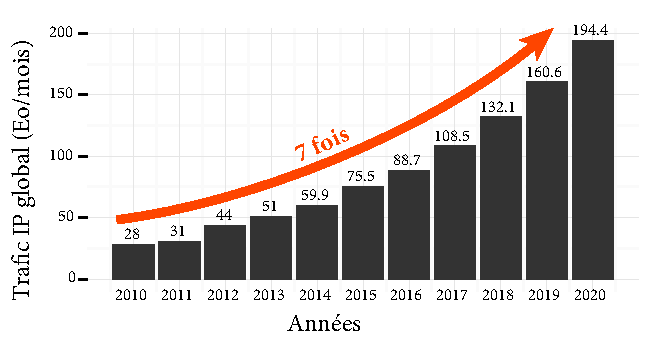
\includegraphics[width=7.5cm]{figures-fr/vni-fr.pdf}
    \vspace{-5pt}
    \caption{Trafic IP global~\cite{index2014forecast}.}
    \label{fig:vni-fr}
\end{wrapfigure}
De nombreux fournisseurs de contenus utilisent déjà des techniques de délestage de données pour livrer du contenu. C’est le cas de Netflix, qui a commencé en 1998 à offrir un service de location de films à ses clients en leur envoyant des DVDs par voie postale.\footnote{\url{http://dvd.netflix.com/}} Il y a quelques années, Amazon a développé le service Import/Export qui permet à ses clients d’envoyer leurs données dans des disques durs par voie postale directement à Amazon, alors en charge de réceptionner les données et de les mettre à disposition dans ses bases de données S3.\footnote{\url{https://aws.amazon.com/fr/importexport/}} Ce service est particulièrement utile pour les clients de Amazon limités par leur connexion Internet à faible débit. Plus récemment, afin de systématiser ces transferts postaux, Amazon a présenté le Amazon Snowball, un appareil portatif prêt à l’envoi et disposant de 50~TB de stockage pour transporter plusieurs Pétaoctets de données vers les bases de données de Amazon. L’ensemble de ces techniques de délestage ont pour but de s’affranchir des limitations actuelles pour transférer de grandes quantités de données, telles que les coûts, la durée ou la sécurité de tels transferts. 

Dans cette thèse, nous proposons d’équiper des véhicules particuliers de capacités de stockage de données pour transformer le réseau routier en un système de transmission à large capacité. Seulement 10\% des véhicules en circulation en France équipés de disques durs de 1~Téraoctets ont le potentiel de transporter 115~Exaoctets de données par jour (ce qui équivaut à 1,3~Petaoctets par seconde). Élargi aux 1,2 milliards de véhicules en circulation dans le monde, la mobilité quotidienne des véhicules représente un potentiel inexploité pour faire face à l’avalanche de données sur les réseaux de données traditionnels tels que l'Internet qui approche. Comme montré sur la Figure~\ref{fig:vni-fr}, les échanges de données ont explosé en triplant ces six dernières années et est prévu de doubler ces cinq prochaines années~\cite{index2014forecast,gantz2012digital,hecht2016bandwidth}. 

L’utilisation opportuniste des véhicules particuliers suit la tendance de services qui reposent sur l’économie partagée tels que Uber ou BlaBlaCar en mettant à disposition le partage de biens et de services de pair à pair. Dans notre cas, les trajets effectués par les véhicules sont les ressources partagées que l’on met à disposition des fournisseurs de contenus pour transporter leurs données. 
 
 
Équiper les véhicules de capacités de stockage de données suit également une tendance actuelle qui crée des services à valeur ajoutée à partir d'un service ``de base''. C’est le cas de services de livraison de colis proposés en complément de services de transportation de passagers. Par exemple, l’américain Greyhound propose un tel service qui repose sur les trajets existants des cars effectués dans le cadre du transport de passagers.\footnote{\url{http://www.shipgreyhound.com/}} De la même manière, l’américain Uber propose UberRUSH, un service de livraison de colis à la demande qui se repose sur une flotte de véhicules normalement dédiés au transport de personnes.\footnote{\url{https://rush.uber.com}} 
 
 
\begin{displayquote} 
    \textit{Dans cette thèse, nous caractérisons et exploitons la mobilité existante d’entités de tous les jours pour atténuer ou s'affranchir des limitations des réseaux de données traditionnels tels que l'Internet. Nous repensons ainsi la conception de services populaires tels que les transferts de données en masse ou les services de partage de données de type ``cloud'' en limitant ou en s’affranchissant de leur dépendance vis-à-vis de ces réseaux.}
\end{displayquote} 
 
 
 
 
\subsection{Vision et conception du service de délestage de données} 
 
 
Nous exploitons la tolérance aux délais du trafic d’arrière-plan pour délester de grandes quantités de données des réseaux de données conventionnels tels que l’Internet vers le réseau routier. En particulier, nous nous intéressons aux transferts de données qui ont lieu dans le cadre d’applications avec une tolérance aux délais de plusieurs jours (par exemple, la distribution de contenus scientifiques ou le trafic d’arrière-plan résultant des activités de maintenance et d’approvisionnement de systèmes distribués large-échelle~\cite{laoutaris2009delay}). Notre délestage de données exploite de manière opportuniste le nombre croissant de trajets de véhicules pour physiquement transporter des données~\cite{le2010mobilite}. 
 
 \begin{figure}[h!]
   \centering
   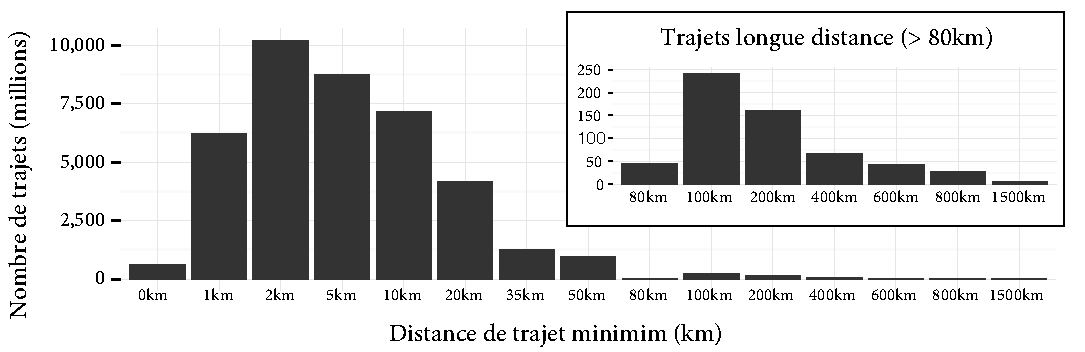
\includegraphics[width=0.9\textwidth]{figures-fr/entd-fr.pdf}
   \caption{Distribution des trajets par distance parcourue par les véhicules en France. Source~: Enquête Nationale Transports et Déplacements (ENTD), 2008~\cite{ENTD}.}
   \label{fig:entd-fr}
\end{figure}
 
Une façon simple de réaliser le délestage de données consiste à utiliser les véhicules qui font l’intégralité du trajet entre la source et la destination du transfert de données. Cependant, comme montré sur la Figure~\ref{fig:entd-fr}, moins de 1,4\% des trajets effectués par des véhicules en France sont long d’au moins 80~km. Bien que cette valeur soit tout de même conséquente pour des transferts sur de courtes distances (cela correspond à environ 600 millions de trajets par an), ce nombre décroit fortement en augmentant la distance des transferts. De plus, en augmentant la portée des transferts, le nombre de destinations différentes augmente, réduisant le nombre de trajets et en laissant juste quelques uns pour livrer les données  sur de longues distances. Une alternative consiste à utiliser une flotte de véhicules dédiés au transport de données de la source du transfert à sa destination. Bien que cette solution n’emploie pas la mobilité existante des véhicules, elle est coûteuse à mettre en place et ne passe pas à l’échelle lorsque le nombre de transferts et de destinations augmente, puisque de plus en plus de véhicules dédiés sont nécessaires. 
 
À la place de ces deux solutions, nous exploitons des facilités dédiées pour composer plusieurs flots de véhicules effectuant des trajets vers différentes directions. Tout au long de cette thèse, nous appellerons ces facilités des \textit{points de délestage}, comme représentés sur la Figure~\ref{fig:offloading-service-architecture-fr}. Ces points de délestage sont équipés de capacités de stockage pour stocker de manière temporaire les données provenant de véhicules s’y arrêtant et ainsi relayer ces données entre véhicules appartenant à différents flots. Ils sont placés aux endroits où les véhicules s’arrêtent fréquemment et suffisamment longtemps pour transférer de grandes quantités de données. Ces endroits correspondent aux emplacements de parking situés le long des routes ou ceux situés dans des villes ou des supermarchés, ou encore des stations-services ou de chargement de batteries électriques. 
 
 
\begin{figure}[t] 
\centering 
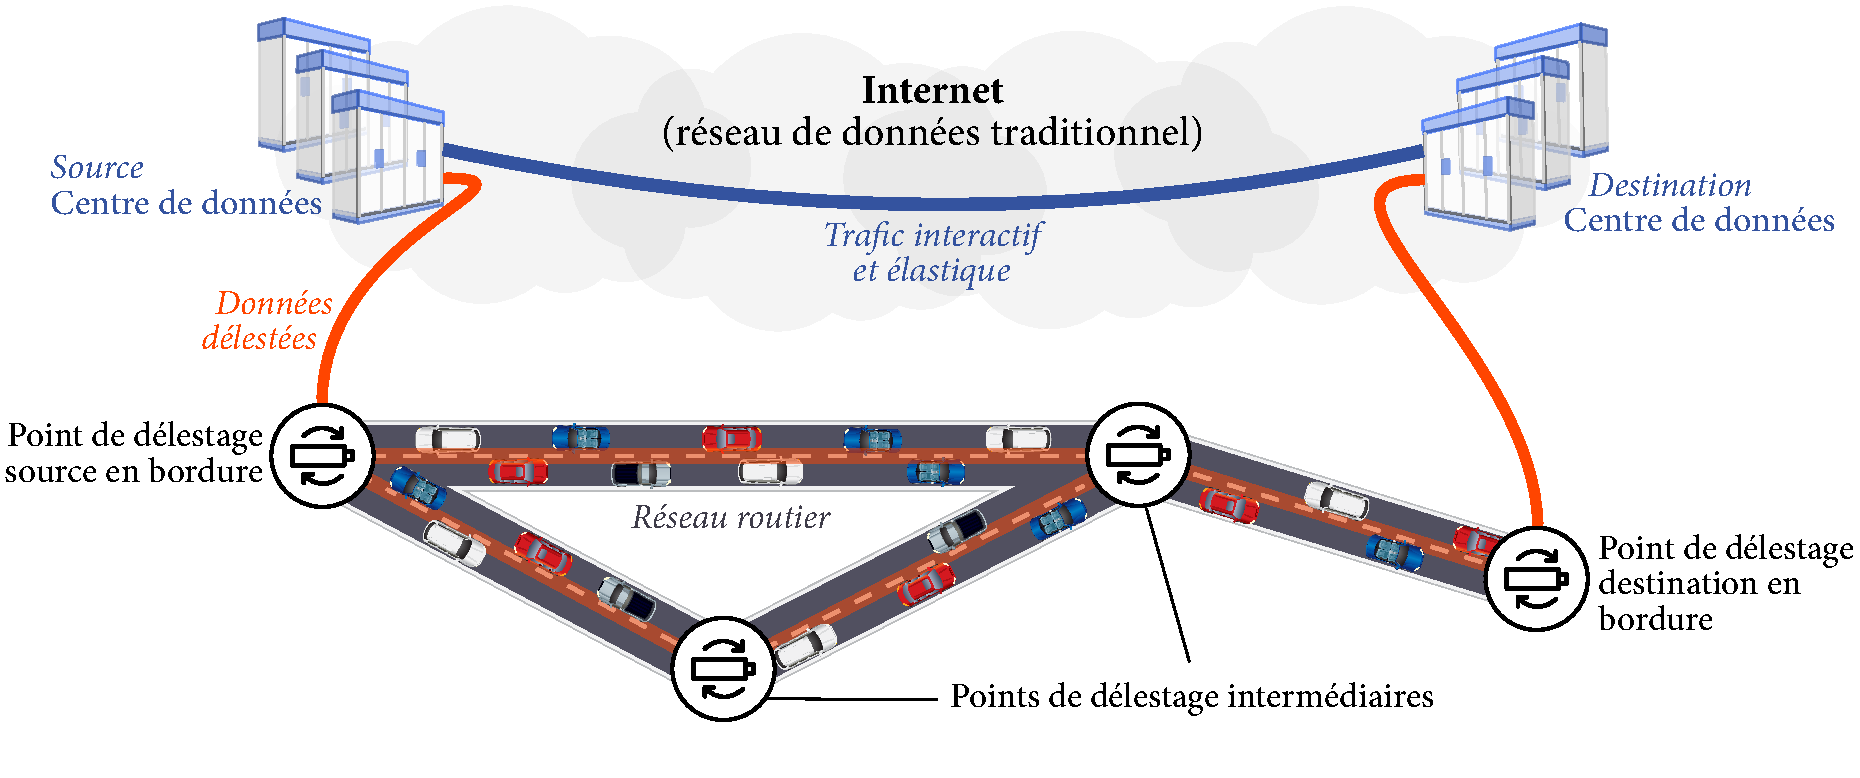
\includegraphics[width=0.9\textwidth]{figures-fr/architecture-2-fr.pdf} 
\caption{Vue générale du délestage de trafic que nous proposons dans cette thèse.} 
\label{fig:offloading-service-architecture-fr} 
\end{figure} 
 
 
À partir de notre travail initial concernant le délestage de données au cœur de cette thèse, nous étendons le concept de point de délestage selon deux directions dans le cadre de services véhiculaires de type ``cloud''. Dans une première extension, nous exploitons la capacité de stockage des points de délestage pour les transformer en dépôts de fichiers et mettre à disposition un système géo-distribué de stockage et de partage de fichiers pour utilisateurs mobiles. Afin d'assurer le partage de fichiers, nous exploitons les mouvements des véhicules entre les points de délestage pour répliquer les fichiers et les rendre accessibles aux utilisateurs. Dans une seconde extension, nous virtualisons les ressources des véhicules afin de créer un réseau véhiculaire mobile. Nous dématérialisons les points de délestage en zones prédéfinies caractérisées par une densité suffisamment élevée de véhicules pour transférer des machines virtuelles entre véhicules. Par ces extensions, nous montrons que la mobilité existante des véhicules a le potentiel de réduire les limitations et la dépendance vis-à-vis des réseaux de données traditionnels. 
 
 
\subsection{Description des problèmes rencontrés} 
 
 
Dans un premier temps, il nous faut allouer de manière efficiente des demandes de délestage de transferts de données aux flots de véhicules existants. Dans la suite de la thèse, nous appelons ce problème le \textit{problème d’allocation de flots de véhicules}. Afin de le résoudre, nous devons créer un processus efficient d’allocation des transferts de données sur des flots de véhicules tel qu’il optimise l'utilisation de ces flots (ressources), tout en satisfaisant les besoins des demandes de délestage correspondantes. 
 
 
\begin{wrapfigure}[15]{o}[0.7\marginparwidth]{6.2cm} 
    \vspace{-10pt} 
    \centering 
    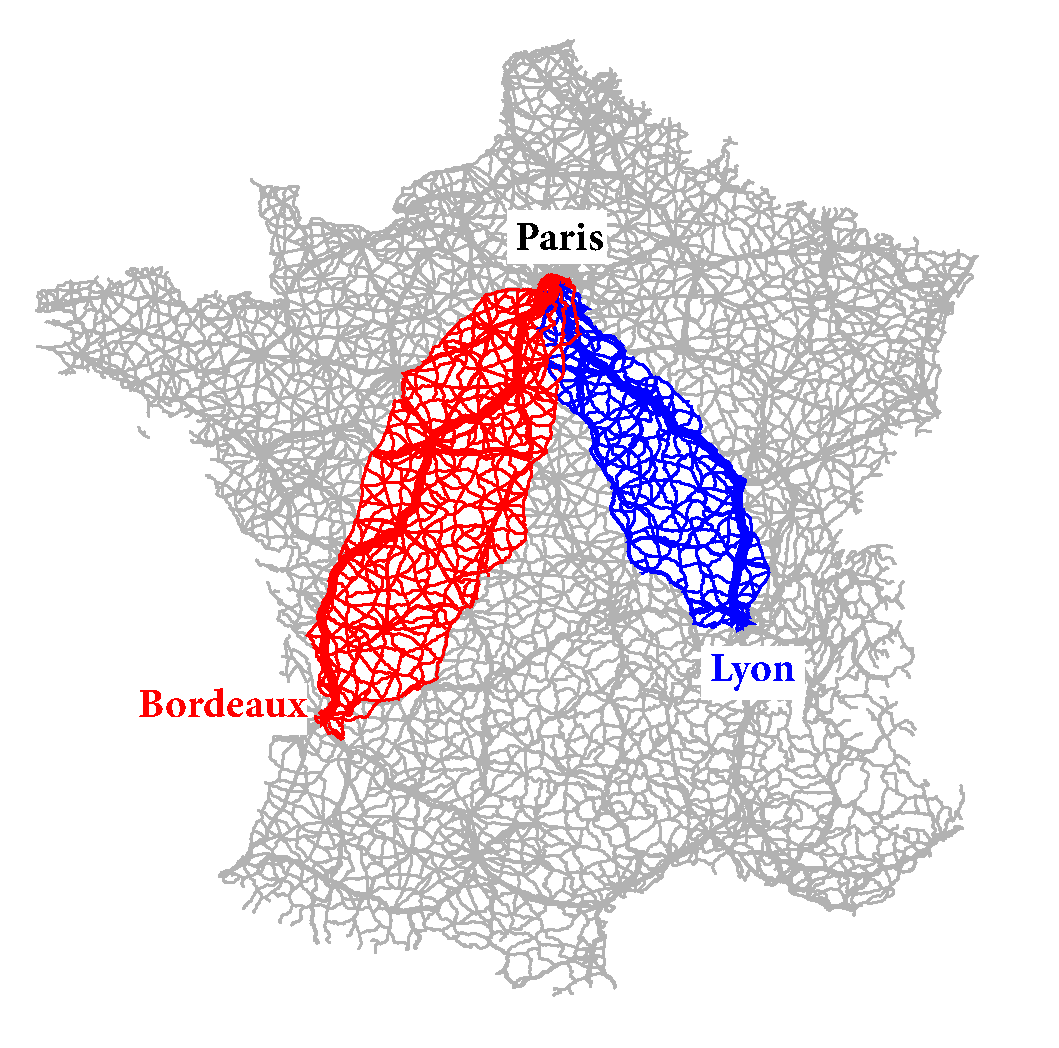
\includegraphics[width=6cm]{figures-fr/france-roads-2.pdf} 
    \caption{Routes principales reliant Paris à Lyon et Bordeaux.} 
    \label{fig:paris-lyon-fr} 
\end{wrapfigure} 
Dans un deuxième temps, il nous faut maîtriser l’échelle du réseau routier afin de pouvoir effectuer un délestage de données qui passe à l’échelle de manière efficiente. En effet, la complexité de la topologie du réseau routier et le grand nombre de trajets effectués rendent le problème d’allocation de flots de véhicules insoluble par calcul. Nous illustrons le besoin d’un mécanisme d’allocation qui passe à l’échelle avec la Figure~\ref{fig:paris-lyon-fr}, où nous représentons les routes des trajets potentiels qui peuvent êtres alloués pour délester des transferts de Paris vers Bordeaux et Lyon. 
 
 
Finalement, nous devons assurer des transferts de données fiables. Parce que les véhicules peuvent ne pas délivrer les données qu’ils transportent vers le prochain point de délestage ou la destination finale, nous devons utiliser et adapter des techniques pour recouvrer des données perdues. 
 
 
Dans les extensions du travail initial, le problème commun est de déterminer les emplacements des points de délestage, selon qu’ils soient matérialisés ou pas, et selon les besoins spécifiques des services que nous déployons. 
 
Plus particulièrement, dans le système de partage de fichiers, nous devons concevoir un algorithme pour placer les points de délestage jouant le rôle de dépôts à des emplacements stratégiques de telle façon qu’ils capturent un nombre maximal de requêtes utilisateurs avant qu’elles n’expirent, tout en les connectant avec les mouvements des utilisateurs pour mettre en place la réplication des fichiers au niveau des dépôts. Dans le cas du réseau véhiculaire virtuel, nous devons identifier les emplacements où les véhicules se rencontrent fréquemment et suffisamment longtemps pour transférer de grandes quantités de données, telles que des machines virtuelles. 
 
 
\section{Délestage massif de données sur le réseau routier} 
 
 
Dans ce chapitre, nous proposons d’évaluer l’utilisation des véhicules circulant sur le réseau routier comme technique de délestage, comme illustré sur la Figure~\ref{fig:offloading-operations-fr}. Les véhicules en circulation sont assimilés aux ressources disponibles dans le réseau routier. Les demandes de délestage provoquent des transferts de données, chacun caractérisé par le délai d’acheminement attendu et la quantité de données à transférer. Nous formulons le problème d’allocation de flots de véhicules en allouant les ressources du réseau routier selon une politique tenant compte des contraintes exprimées en termes de délai et de débit qui caractérisent ce transfert. La définition d’une politique d’allocation des ressources est un problème NP-complet et les techniques traditionnelles de réduction ne sont pas applicables en raison de la complexité de la topologie routière et du nombre de véhicules circulant sur les routes. 
 
 
\begin{figure}[h!] 
    \centering 
    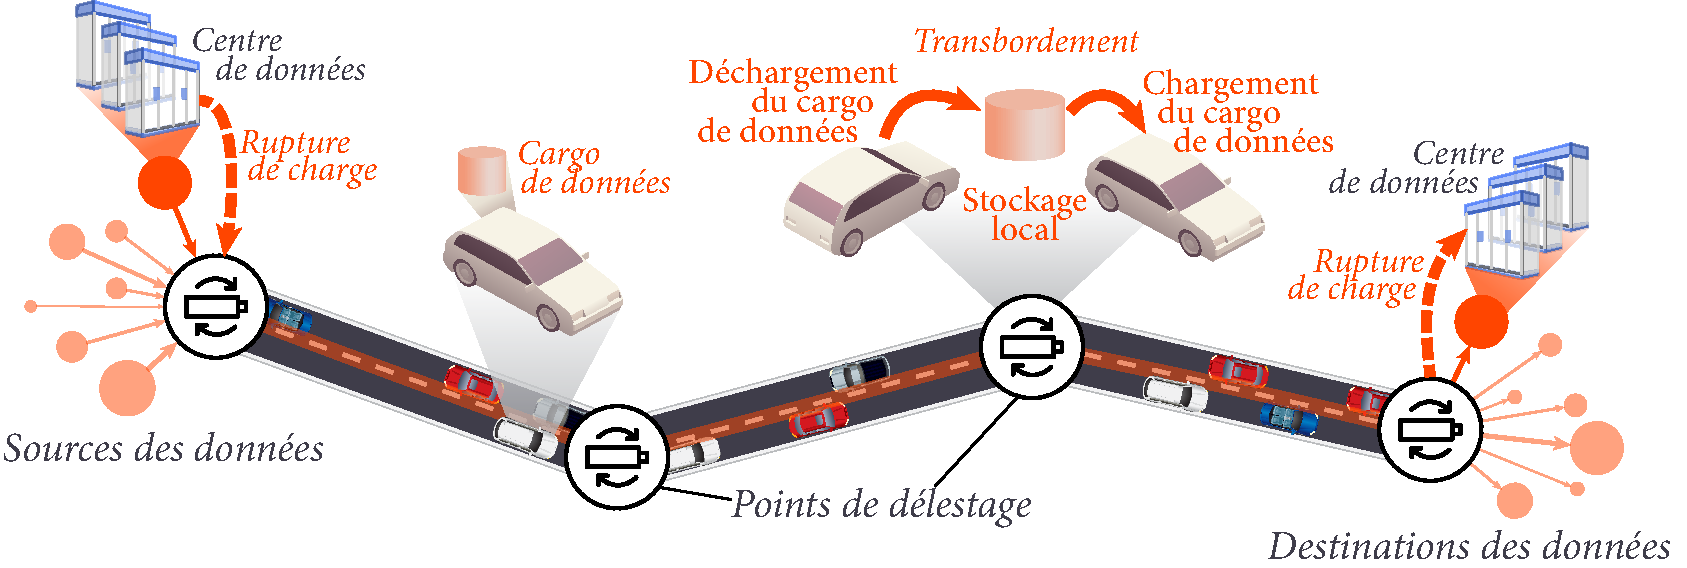
\includegraphics[width=0.95\columnwidth]{figures-fr/taxonomy-fr.pdf} 
    \caption{Overview of the operations to offload large amounts of data over the road network.} 
    \label{fig:offloading-operations-fr} 
\end{figure} 
 
 
Afin de contourner cette complexité, nous employons une approche en deux phases. D’une part, nous simplifions le réseau routier en construisant un réseau de recouvrement, appelé ``réseau de délestage'' qui offre une vue logique du réseau routier sous-jacent (Figure~\ref{fig:France-overlay-fr}). En éliminant un grand nombre de routes inutiles, la complexité due à la taille du réseau est mieux maîtrisée. D’autre part, nous proposons une formulation de l’allocation des flots de véhicules par un algorithme max-min équitable utilisant des modèles de programmation linéaire pour déterminer les chemins logiques optimaux pour le transport des données délestées (Section~\ref{sec:modele-delestage-fr}). Enfin, nous évaluons la capacité de notre système de délestage sur l’infrastructure routière française avec des données de trafic routier réelles (Section~\ref{sec:evaluation-fr}). 
 
\subsection{Architecture centralisée pour le délestage de données utilisant les véhicules} 
 
Dans cette section, nous donnons une vue globale des opérations de l’infrastructure en charge de délester les données. Nous nous intéressons à des transferts qui durent plusieurs jours engendrés par des activités de maintenance ou d’approvisionnement pour des migrations de machines virtuelles ou des sauvegardes hors-ligne entre centres de données (\textit{data centers} en anglais). La figure~\ref{fig:offloading-operations-fr} montre les opérations de notre infrastructure de délestage sur un fragment de réseau routier. 

Des véhicules particuliers sont équipés de disques durs leur permettant de stocker des données. De plus, les véhicules sont équipés d’interfaces de communication pour échanger des données à haut débit. 

Le flot de véhicules ainsi équipés joue le rôle d’un \textit{backhaul} mécanique qui connecte une collection de points de délestage, comme montré sur la Figure~\ref{fig:offloading-operations-fr}. Les points de délestage ont deux rôles selon leur position relative dans le processus de délestage. Ce double rôle est montré sur la Figure~\ref{fig:offloading-operations-fr}. Une partie ou tout le trafic de données provenant d’un réseau de données traditionnel est premièrement \textit{dévié} de ce réseau vers le plus proche point de délestage en bordure du transfert (rupture de charge). Les données sont temporairement stockées dans le point de délestage et chargées sur les véhicules s’y arrêtant. Les points de délestage suivants sont alors en charge de relayer les données en les \textit{transbordant}. Les véhicules déchargent les données qu’ils transportent pendant leur arrêt aux points de délestage. Les données sont temporairement stockées jusqu’à ce qu’un véhicule ne les charge lors de son arrêt et les transporte jusqu’au point de délestage suivant. Une fois arrivées au point de délestage destination en bordure, les données sont à nouveau déviées vers le réseau de données traditionnel. 
 
 
Pour implémenter le délestage de données sur le réseau routier, nous exploitons les avantages d’une centralisation logique en utilisant une architecture de type SDN (\textit{Software-Defined Networking}) qui permet un contrôle efficient et une gestion de l’infrastructure de délestage. En effet, le concept de SDN fournit les moyens logistiques, en particulier la planification, l’orchestration, l'implémentation et lecontrôle pour mettre en place le délestage de données~\cite{mckeown2008openflow}. 
 
 
L’architecture centralisée comprend un contrôleur central et une collection de points de délestage qui agissent comme des commutateurs en acheminant les données.  
 
 
Afin d’assurer le fonctionnement en continu du service de délestage, le contrôleur surveille le fonctionnement des points de délestage, en particulier la quantité d’espace de stockage disponible et les destinations des données en transbordement. Pour améliorer les décisions d’acheminement des données en prédisant la future destination des véhicules, le fournisseur de service récupère l’itinéraire suivi par les véhicules qui s’arrêtent aux points de délestage via leur système de navigation.  
 
 
Le contrôleur reçoit les demandes pour délester des données et est en charge d’assigner les transferts à des chemins routiers et les flots de véhicules correspondants. Un chemin routier correspond aux flots de véhicules successifs qui connectent une séquence de points de délestage. Le contrôleur détermine ces chemins en résolvant le problème d’allocation de flots de véhicules qu’on formule avec un modèle max-min équitable dans la Section~\ref{sec:modele-delestage-fr}. Cette formulation maximise le débit résultant de l’allocation des transferts de données tout en la garantissant équitable afin d’éviter les famines pour les transferts alloués. Le résultat du problème est ensuite utilisé pour configurer la séquence de points de délestage participant aux transferts alloués.  
 
 
\subsection{Modèle économique avec les véhicules électriques} 
 
\begin{figure}[h!]
    \centering
    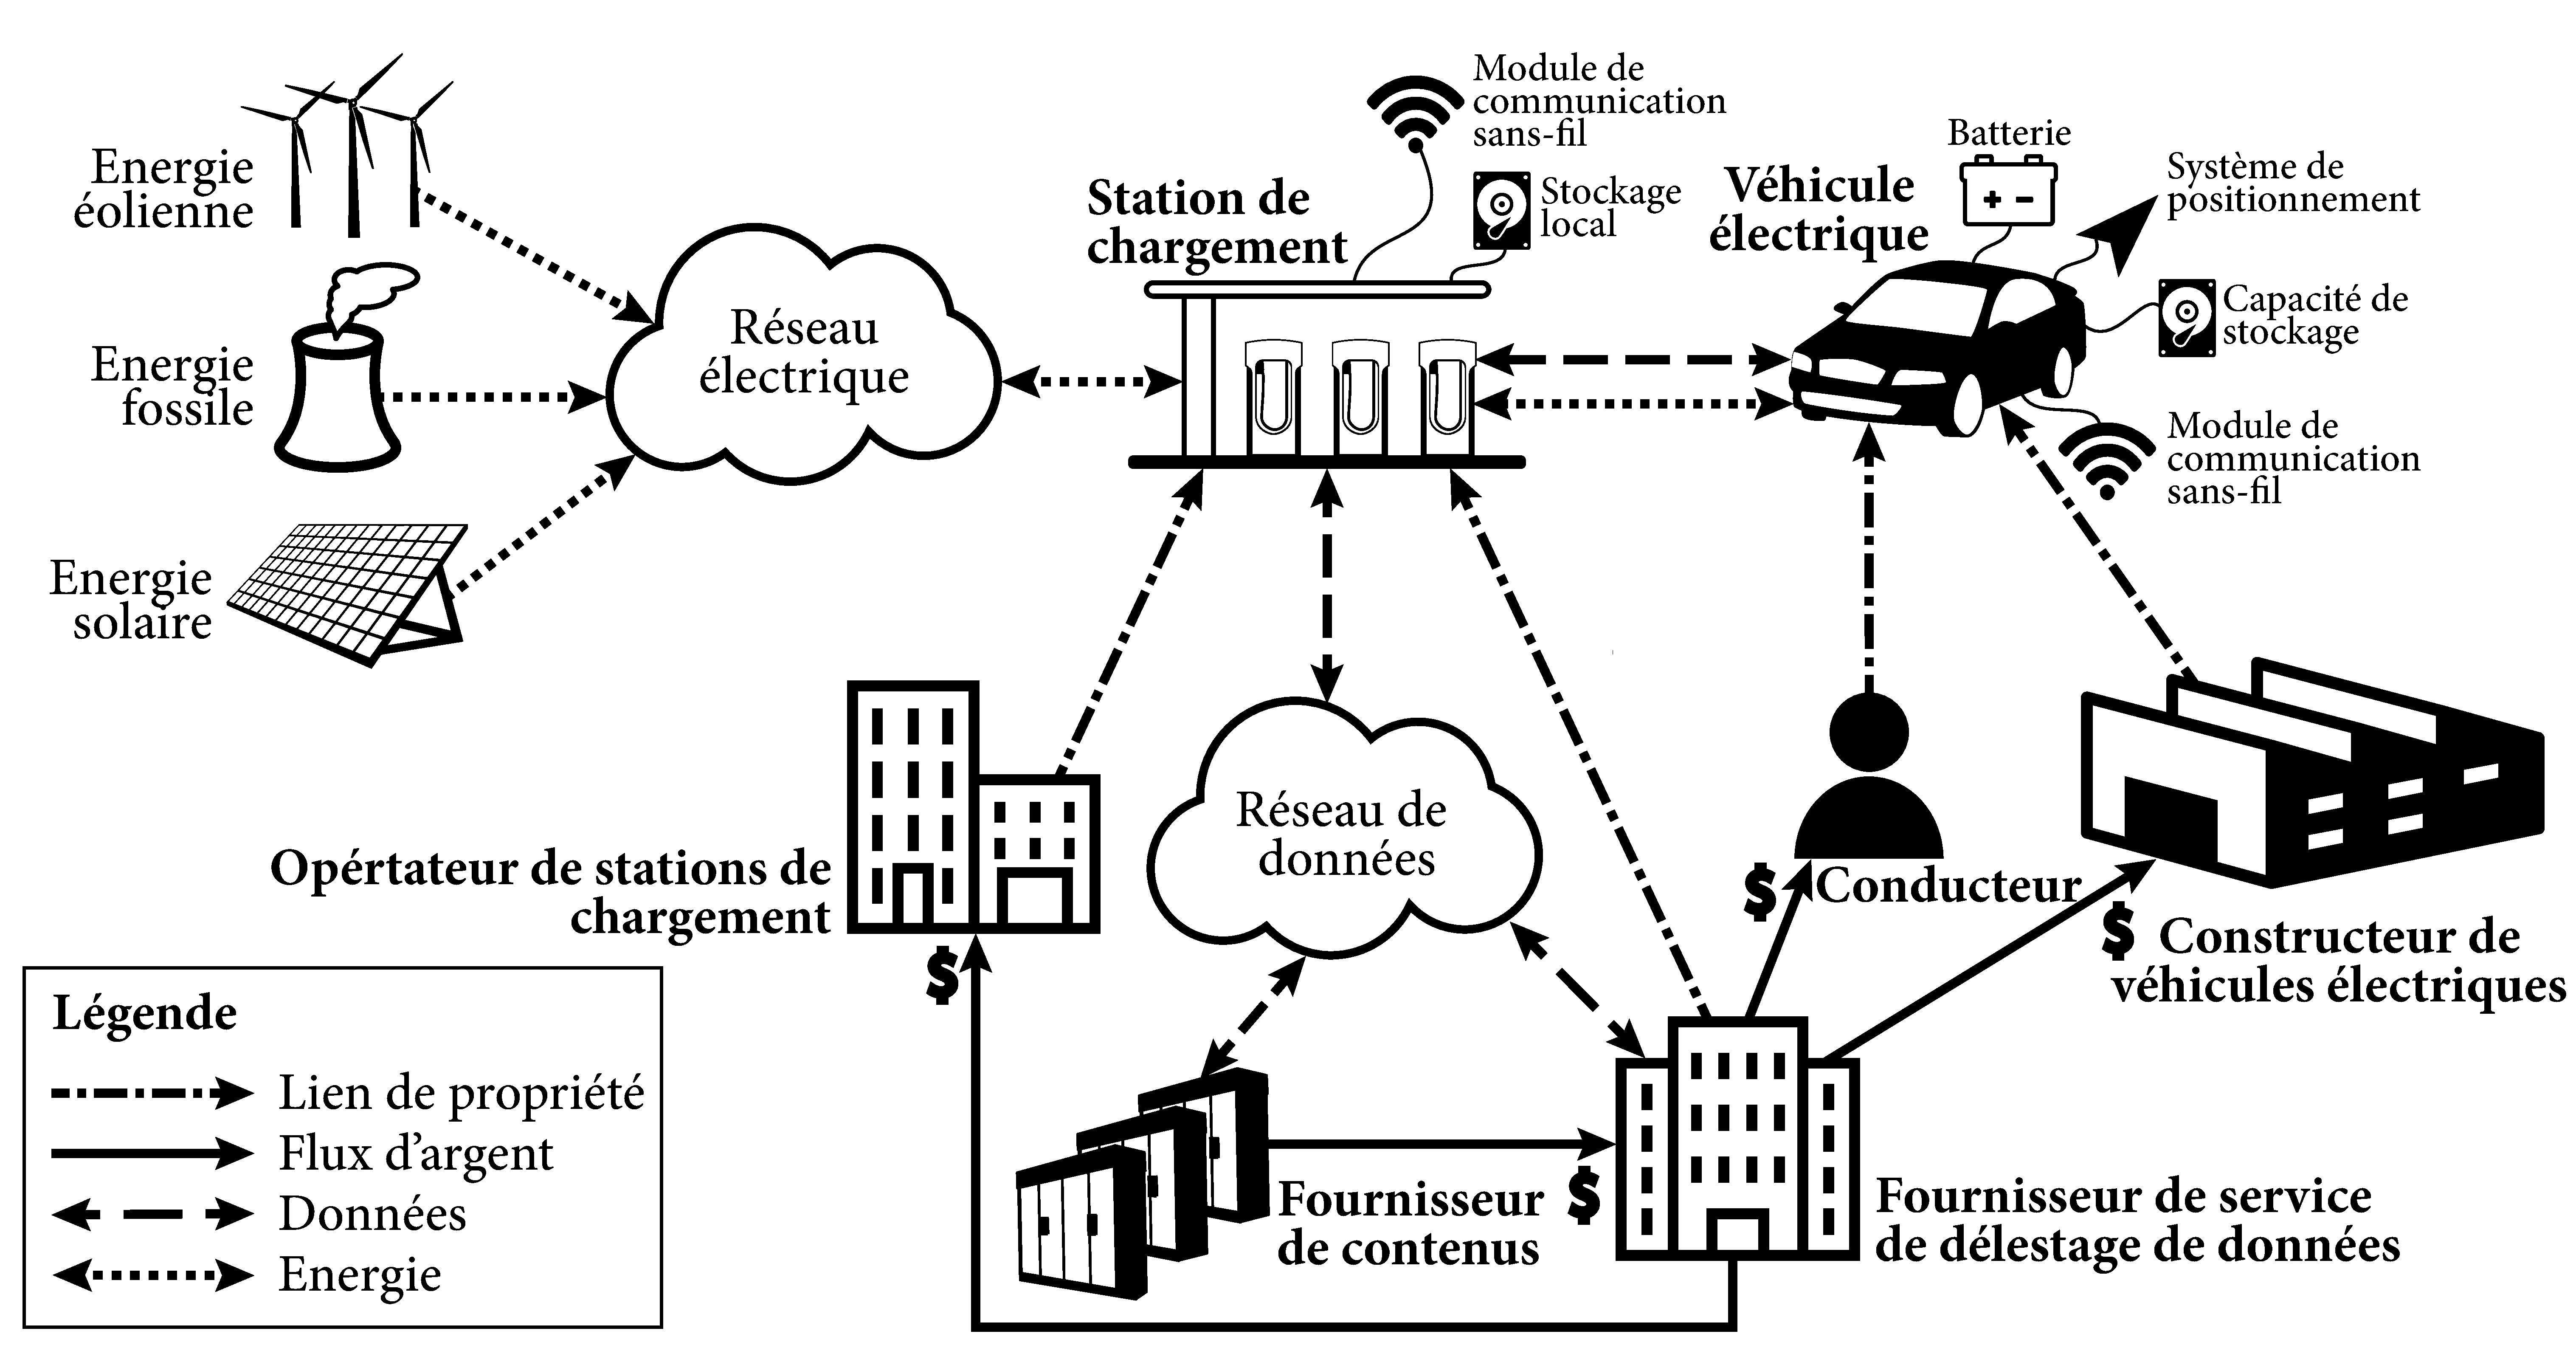
\includegraphics[width=0.9\textwidth]{figures-fr/business-plan-fr.pdf}
    \caption{Modèle économique du délestage de données.}
    \label{fig:business-model-fr}
\end{figure}

Dans cette section, nous présentons le le modèle économique que l’on utilisera dans la suite de cette thèse. Ce modèle inclut (\textit{i}) des véhicules électriques et leur conducteurs, (\textit{ii}) un fournisseur de service de délestage de données (qui peut être le constructeur de véhicules électriques), (\textit{iii}) un opérateur de stations de chargement de batteries de voitures électrique, et enfin (\textit{iv}) un fournisseur de contenus qui opère plusieurs centres de données géo-distribués. 
 
 
En particulier, ce modèle nous permet de modéliser et analyser ce que nous proposons dans des conditions réalistes en se basant sur des éléments qui nous permettent de réaliser le délestage de données sur le réseau routier tels que la portée des véhicules électriques qui permet d’avoir des arrêts fréquents ou le temps de chargement de batteries électriques qui permet de transférer de grandes quantités de données pendant le temps de chargement de la batterie.
 
 
Dans le cadre de ce scénario, les véhicules électriques sont équipés de capacités de stockage de données et les stations de chargement de batteries électriques jouent le rôle de points de délestage permettant de charger ou décharger les données des véhicules pendant la charge de leur batterie. Le fournisseur du service de délestage utilise et gère le contrôleur central présenté dans la section précédente. 
 
 
Le fournisseur de service de délestage de données, si différent du constructeur de véhicules électriques, propose des compensations financières aux conducteurs pour effectuer leurs trajets habituels à condition de transporter un disque dur à bord de leur véhicule. La compensation financière est déterminée avec l’opérateur de stations de chargement de batteries électriques en fonction du nombre de kilomètres parcourus et de la couverture effective. Dans le cas où le constructeur de véhicules électriques a le rôle du fournisseur de service de délestage de données, les véhicules sont équipés de série avec des disques durs et le service est fourni sans compenser les conducteurs. Le fournisseur de service de délestage de données facture le fournisseur de contenus en fonction de la quantité de données délestée sur le réseau routier et partage les revenus avec l’opérateur de stations de chargement. 
 
 
Une fois les demandes de délestage de transferts de données émises par des fournisseurs de contenus, le fournisseur de service de délestage détermine la quantité de données à allouer à chaque flot de véhicules se déplaçant entre les points de délestage. 
 
 
\subsection{Motivation pour avoir un contrôleur centralisé} 
\label{sec:scenario-simple-fr} 
 
 
Dans cette section, nous présentons un exemple de réseau routier volontairement simple pour montrer les bénéfices d’un contrôleur centralisé. Le réseau routier est représenté sur la Figure~\ref{fig:simple-scenario-fr} et comporte quatre points de délestage. Nous comparons deux stratégies d’ordonnancement implémentées au niveau du point de délestage $S$. Nous considérons deux transferts de données $A$ et $B$ provenant tous deux de $S$, partageant tous deux le tronçon $I$ et allant à leurs destinations finales respectives $T_A$ et $T_B$. Nous considérons seulement le trafic routier des tronçons représentés sur la figure. 
 
 
\begin{figure}[ht] 
    \centering 
    \begin{subfigure}[t]{0.45\columnwidth} 
        \centering 
        % \raisebox{.2\textwidth}{ 
        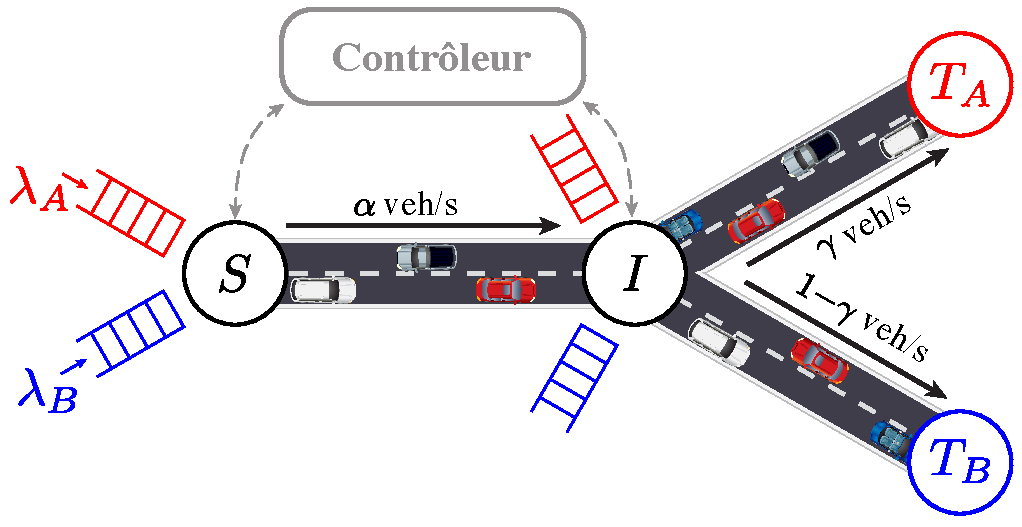
\includegraphics[width=\textwidth]{figures-fr/simpleScenario-fr.pdf} 
        % } 
        \caption{Deux transferts de données $A$ et $B$ provenant tous deux de $S$ partagent le tronçon $I$ et suivent leur route jusqu’à leurs destinations respectives $T_A$ et $T_B$.} 
        \label{fig:simple-scenario-fr} 
    \end{subfigure}% 
    \quad %add desired spacing between images, e. g. ~, \quad, \qquad etc. 
      %(or a blank line to force the subfigure onto a new line) 
    \begin{subfigure}[t]{0.51\columnwidth} 
        \centering 
        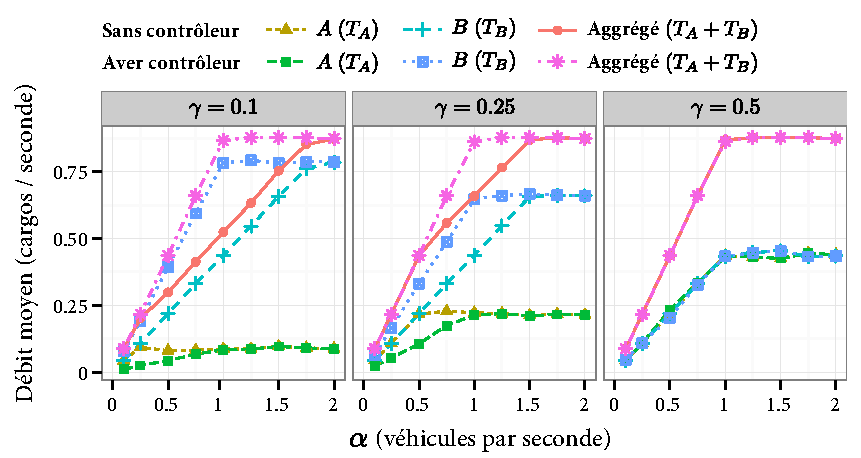
\includegraphics[width=\textwidth]{figures-fr/simpleScenario-throughput_v2_gamma_all-fr.pdf} 
        \caption{Débit maximal (exprimé en nombre de cargos de données délivrés par seconde) pour les deux stratégies d’ordonnancement en fonction des deux paramètres $(\alpha,\,\gamma)$.} 
        \label{fig:simple-scenario-throughput-fr} 
    \end{subfigure} 
    \caption{Réseau routier composé de quatre points de délestage afin de montrer les bénéfices résultant d’un contrôleur.} 
\end{figure} 
 
 
Nous considérons deux stratégies d’ordonnancement implémentées au niveau du point de délestage $S$: (\textit{i}) sans contrôleur et (\textit{ii}) avec contrôleur. Elles permettent de sélectionner les cargos de données issus d’un transfert de données (soit $A$, soit $B$) à charger sur chaque véhicule s’arrêtant au point de délestage $S$. La première stratégie (sans contrôleur) suit un ordonnancement de type ``Round-Robin'' en sélectionnant les données dans les mêmes proportions et en ordre circulaire, sans donner de priorités aux transferts. La seconde stratégie (avec contrôleur) utilise un contrôleur pour définir des configurations à installer au niveau du point de délestage $S$ pour effectuer la décision pondérée de sélection du transfert et du cargo de données à charger dans le véhicule à l’arrêt. Le contrôleur détermine cette configuration avec des poids proportionnels aux volumes de trafic routier sur les différents tronçons. Ainsi, si l’on considère un trafic routier trois fois plus important sur le tronçon $(I,\,T_A)$ par rapport au tronçon $(I,\,T_B)$, la seconde stratégie va charger trois fois plus de données sur les véhicules en direction de $T_A$. Ce n’est pas le cas de la première stratégie~: celle-ci va charger les mêmes quantités de données sur les véhicules qu’ils aillent en direction de $T_A$ ou de $T_B$. 
 
 
Nous utilisons SUMO pour évaluer les deux stratégies d’ordonnancement~\cite{behrisch2011sumo}. À l’aide de ce simulateur, nous simulons le trafic routier avec des volumes de (\textit{i}) $\alpha$ véhicules par seconde de $S$ vers $I$, (\textit{ii}) $\gamma$ de $I$ vers $T_A$, et (\textit{iii}) $1 - \gamma$ de $I$ vers $T_B$. Nous supposons que chacun des deux transferts $A$ et $B$ a une quantité de données infinie à transporter de $S$ vers $T_A$ et $T_B$, respectivement (\ie $\lambda_A = \lambda_B = \infty$). La Figure~\ref{fig:simple-scenario-throughput-fr} montre le débit du système mesuré en terme de nombre de cargos de données livrés à la destination par seconde.  
 
 
Nous constatons qu’avec la première stratégie (sans contrôleur), le transfert $A$ a besoin de plus de débit routier ($\alpha$) pour atteindre son débit nominal. Sans connaissance du trafic routier en aval, $S$ ne peut pas charger les quantités optimales de données au prochain point de délestage de telle façon que $I$ utilise pleinement les ressources véhiculaires. De ce fait, $I$ n’a pas assez de données disponibles localement pour alimenter le flot routier à destination de $T_B$. Les ressources disponibles sur le tronçon $(I,\,T_B)$ restent sous-utilisées si les cargos de données ne sont pas transportés en nombre adéquat de $S$ vers $I$ (par exemple, $\alpha = 2$). Au contraire, la seconde stratégie avec contrôleur permet de transporter un nombre adéquat de cargos de données de $S$ vers $I$. De ce fait, $I$ a suffisamment de données à disposition pour utiliser pleinement les véhicules en direction de $T_A$ et $T_B$. Le contrôleur utilise sa connaissance du trafic routier en aval pour maximiser l’utilisation des ressources au niveau du point de délestage $S$. Cette stratégie donne un meilleur débit pour chacun des transferts en compétition au niveau de $S$. 
 
 
À l’aide de cet exemple simple, nous avons montré les bénéfices d’une architecture centralisée qui pré-configure les points de délestage afin d’effectuer des décisions pondérées pour charger les données sur les véhicules à l’arrêt. Cette architecture permet d’avoir de meilleurs débits par rapport à une architecture distribuée où les décisions de chargement de données sur les véhicules sont faites de manière locale.  
 
 
 
 
\subsection{Allocation des flots de véhicules pour des transferts de données délestés sur le réseau routier} 
\label{sec:modele-delestage-fr} 
 
 
Le problème d’allocation de flots de véhicules revient à déterminer les routes suivies par les données transportées par les flots de véhicules entre les points de délestage. Avant de résoudre ce problème, il nous faut nous affranchir de la complexité du réseau routier de par la taille et la couverture de sa topologie et de par le nombre de trajets véhiculaires qui rendent le problème insoluble par calcul.  
 
 
Dans cette section, nous présentons un algorithme pour réduire la complexité du réseau routier. Le résultat de cet algorithme est un réseau de délestage en sur-couche qui est une représentation logique du réseau routier et en capture ses principales caractéristiques qui nous sont nécessaires pour résoudre le problème d’allocation de flots de véhicules. 
 
 
\subsubsection{Notations préliminaires} 
 
 
\paragraph{Réseau routier.}  
Nous représentons le réseau routier par un graphe orienté composé de tronçons de routes (les liens) et d’intersections (les nœuds). Les points de délestage correspondent également à des nœuds et sont situés aux intersections ou le long des tronçons. Pour un tronçon $(a,\,b)$, nous définissions par $v_{ab}$ le volume nominal de véhicules (en terme de nombre de véhicules par unité de temps), par $c_{ab}$ la capacité du tronçon (également en terme de nombre de véhicules par unité de temps), et par $t_{ab}(v_{ab})$ le temps de trajet, fonction du volume nominal de véhicules. 
 
 
Nous utilisons des jeux de données qui comportent les volumes de trafic sur les tronçons de route exprimés par des Trafic Moyens Journaliers Annuels (TMJA). Le TMJA est le volume de trafic total mesuré traversant un tronçon de route dans les deux sens pendant une année divisé par le nombre de jours dans l’année. De ce fait, la capacité $c_{ab}$ du tronçon $(a,\,b)$ est fixée à la valeur du TMJA pour ce tronçon dans le jeu de données. 
 
\begin{wrapfigure}[15]{o}[0.7\marginparwidth]{7.5cm}
    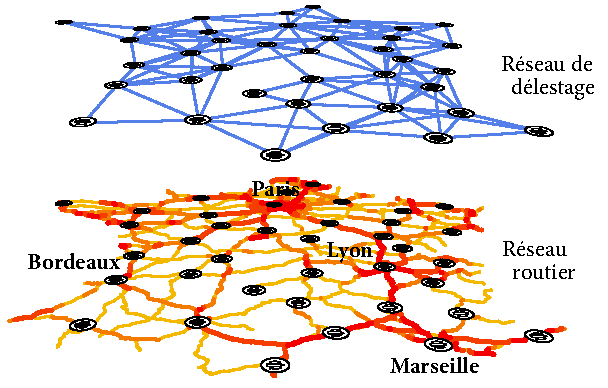
\includegraphics[width=7cm]{figures-fr/France-overlay-fr.pdf}
    \caption{Le réseau de délestage représenté au dessus du réseau routier français. Le réseau de délestage résulte d’un déploiement de stations de chargement de batteries électriques couvrant le réseau routier français.}
    \label{fig:France-overlay-fr}
\end{wrapfigure}
\paragraph{Réseau de délestage en surcouche.} 
Afin de nous affranchir de la complexité du réseau routier, nous proposons un algorithme de réduction du réseau routier. Notre algorithme construit un réseau de recouvrement, appelé \textit{réseau de délestage}, qui offre une vue logique simplifiée du réseau routier sous-jacent. Le réseau de recouvrement est représenté par un graphe orienté noté $G^{O}$, où les nœuds $N^{O}$ sont les points de délestage. Les liens logiques $L^{O}$ qui connectent les points de délestage résultent de l’agrégation  des tronçons du réseau routier $G^{R}$ sous-jacent. Un lien logique $(i,\,j)$ de $L^{O}$ est caractérisé par sa capacité $c(i,\,j)$ calculée en fonction du trafic routier, son délai de propagation $t(i,\,j)$ qui représente le temps de trajet moyen le long des routes sous-jacentes et par un taux d’erreur $l(i,\,j)$. Le taux d’erreur correspond à la proportion des véhicules n’arrivant pas à destination en raison de prédictions erronées de la future direction des véhicules lors de leurs arrêts aux points de délestage. 
 
 
\subsubsection{Caractérisation du réseau de délestage en surcouche} 
 
 
Dans cette section, nous caractérisons les liens logiques du réseau de délestage en surcouche par des quantités réseau afin de résoudre le problème d’allocation de flots de véhicules. 
 
 
\paragraph{Temps de trajet $t(i,\,j)$.} 
Le temps de trajet $t_{ab}$ du tronçon $(a,\,b)$ est donné par la fonction définie par le BPR (\textit{Bureau of Public Roads} aux États-Unis) par~: 
\begin{equation} 
  \label{eq:BPR-fr} 
  t_{ab}(v_{ab})=t_{ab}(0)\left[1+\alpha\left(\frac{v_{ab}}{c_{ab}}\right)^{\beta}\right]\Comma 
\end{equation} 
\noindent où $\alpha$ et $\beta$ sont des paramètres définis par le BPR qui dépendent du profil de la route (typiquement $\alpha = 0.15$ minutes et $\beta = 4.0$)~\cite{HCM00}. 
 
 
De l’Équation~\ref{eq:BPR-fr}, nous pouvons en déduire le temps de trajet sur le chemin routier $p$, noté $t_{p}$, qui correspond à la somme des temps de trajet des tronçons qui composent le chemin (sans considérer les délais aux intersections)~:
\begin{equation} 
  \label{eq:path-delay-fr} 
  t_{p} = \sum_{(a,\,b)\in p} t_{ab}(v_{ab}). 
\end{equation} 
 
 
De l’Équation~\ref{eq:path-delay-fr}, nous en déduisons une expression du temps de trajet $t(i,\,j)$ sur les $r$ chemins routiers entre $i$ et $j$, pondéré par les volumes de trafic routier $v_{p}$ sur chacun des chemins $p$. 
 
 
\begin{equation} 
  t(i,\,j) = \frac{\sum_{p\in S_{ij}} t_{p}\,v_{p}}{r\sum_{p\in S_{ij}}v_{p}}\Comma 
\end{equation} 
\noindent où $S_{ij}$ correspond à l’ensemble des chemins routiers entre $i$ et $j$, sans cycles. 
 
 
 
 
\paragraph{Capacité $c(i,\,j)$.} 
La capacité $c(i,\,j)$ du lien logique $(i,\,j)\in L^{O}$ est fonction de la somme des volumes de trafic $v_{p}$  des chemins routiers entre les points de délestage $i$ et $j$ (\ie le nombre de véhicules par unité de temps allant de $i$ à $j$ sur le chemin routier $p$). La capacité du lien logique est également fonction du taux de pénétration de marché $\mathcal{M}$ des véhicules participant au délestage de données et de la capacité de stockage des véhicules $\mathcal{S}$ (nous supposons que tous les véhicules sont équipés de disques durs de même capacités $\mathcal{S}$). 
 
 
\begin{equation} 
  c(i,\,j) = \mathcal{M} \mathcal{S} \sum_{p\in \mathcal{P}^{ij}} v_{p}. 
\end{equation} 
 
 
Dans l’évaluation des performances présentée dans la Section~\ref{sec:evaluation-fr}, nous déduisons la valeur de $v_{p}$ pour chacun des chemins $p$ à partir du jeu de données du réseau routier français. Ce jeu de données contient des comptages de trafic routier réels pour chacun des tronçons dont chaque chemin $p$ est constitué. 
 
 
\paragraph{Taux d’erreur $l(i,\,j)$.} 
Le taux d’erreur $l(i,\,j)$ (compris entre 0 et 1) du lien logique $(i,\,j)$ représente la proportion de données perdues entre les points de délestage $i$ et $j$. Comme mentionné précédemment, ces pertes sont dues aux erreurs de prédictions des futures directions des véhicules lors de leurs arrêts aux points de délestage.  
 
 
\paragraph{Demandes de délestage.} 
Une demande de délestage $d_{st}$ entre deux points de délestage $s$ et $t$ est caractérisée par la quantité de données à transférer $\beta_{st}$ et un délai imparti pour transporter ces données $\tau_{st}$. Par simplification, nous modélisons le taux des demandes arrivant à la source $s$ par une distribution de Poisson $\lambda_{st}$ avec un débit moyen de $\beta_{st}/\tau_{st}$. 
 
 
Pour améliorer la lisibilité, nous donnons les notations utilisées dans la Table~\ref{tab:main-variables-haulage-fr}. 
 
 
\begin{table}[ht] 
    \caption{Table des notation utilisées pour l’algorithme d’allocation max-min équitable.} 
    \renewcommand{\arraystretch}{1.1} 
    \centering 
    {\footnotesize 
    \begin{tabular}{c|l} 
        \textbf{Variable} & \textbf{Signification}\tabularnewline 
        \hline  
        $d_{st}$ & Demande de délestage entre la source $s$ et la destination $t$\tabularnewline 
        $\tau_{st}$ & Temps imparti pour transférer les données de la demande de délestage $d_{st}$\tabularnewline 
        $\beta_{st}$ & Quantité de données à transférer pour la demande de délestage $d_{st}$\tabularnewline 
        $\lambda_{st}$ & Taux d’arrivées Poissonniennes à la source $s$ de la demande de délestage $d_{st}$\tabularnewline 
        $\mathcal{P}_{st}$ & Ensemble de chemins logiques entre $s$ et $t$ sur le réseau de délestage\tabularnewline 
        $\mathcal{S}$ & Capacité de stockage des véhicules\tabularnewline 
        $\mathcal{M}$ & Taux de pénétration de marché\tabularnewline 
        $c\left(i,\, j\right)$ & Capacité du lien logique $\left(i,\, j\right)$\tabularnewline 
        $t\left(i,\, j\right)$ & Temps de trajet sur le lien logique $\left(i,\, j\right)$\tabularnewline 
        $l\left(i,\, j\right)$ & Taux d’erreur du lien logique $\left(i,\, j\right)$\tabularnewline 
        $l^{\textrm{\textbf{red}}}_{st}\left(i,\, j\right)$& Taux d’erreur sur le lien logique $\left(i,\, j\right)$ avec redondance pour la demande de délestage $d_{st}$\tabularnewline 
        $O^{\textrm{\textbf{red}}}_{st}$ & Quantité additionnelles transmises dues au mécanisme de \textbf{red}ondance sur le flot de données\\
         & pour la demande de délestage $d_{st}$\tabularnewline 
        $R^{\{\textrm{hbh,e2e}\}}_{st}(i,\,j)$ & Nombre moyen de transmissions (soit de bout-en-bout (\textbf{e2e}) ou saut-à-saut (\textbf{hbh}) \\ 
         & pour un cargo de données sur le lien logique $(i,\,j)$ pour la demande de délestage $d_{st}$\tabularnewline 
        $\delta_{i}$ & Temps d’attente au point de délestage $i$ (pour recharger la batterie du véhicule électrique)\tabularnewline 
        $f\left(p\right)$ & Flot de données sur le chemin logique $p$\tabularnewline 
        $t\left(p\right)$ &  Temps de trajet du chemin logique $p$\tabularnewline 
        $O_{st}(i,\,j)$ & Données additionnelles pour la demande de délestage $d_{st}$ sur le lien logique $(i,\,j)$\tabularnewline 
        $R_{st}(i,\,j)$ & Nombre de transmission d’un cargo de données sur le lien logique $(i,\,j)$ \\
         & indépendamment du mécanisme de retransmission utilisé\tabularnewline 
    \end{tabular}} 
    \label{tab:main-variables-haulage-fr} 
\end{table} 
 
 
\subsubsection{Fiabilité des transferts délestés} 
\label{sec:fiabilite-fr} 
 
 
Dans cette section, nous présentons les deux mécanismes que nous utilisons pour fiabiliser les communications et leur impact sur la quantité de données additionnelles à transférer (\textit{overhead} en anglais). 
 
 
Les taux d’erreur des liens empruntés sont absorbés pour obtenir des transferts fiables en appliquant les deux méthodes suivantes~: (\textit{i}) encodage des données selon des techniques de sur-échantillonnage qui procèdent par ajout de redondance (par exemple, RAID) et (\textit{ii}) retransmission des données perdues sur un lien logique depuis le point de délestage précèdent (par exemple, SR-ARQ~\cite{costello2004error}). Ces deux méthodes augmentent la quantité de données à transporter par un facteur multiplicatif noté respectivement $o_{st}^{\text{red}}$ pour les techniques de redondance et  $o_{st}^{\text{ret}}$ pour celles basées sur la retransmission des données.  
 
 
\paragraph{Redondance des cargos de données.} 
L’utilisation de la redondance permet néanmoins de réduire les pertes sur chaque lien logique, dont le taux de perte passe de $l(i,\,j)$ à $l^{\text{red}}_{st}(i,\,j)$. Nous utilisons la redondance avec RAID~6 qui arrange les cargos de données en ensembles de $n$ cargos ($n\geq$), incluant deux cargos redondants (et $n-2$ cargos utiles). Le nouveau taux de perte $l^{\text{red}}_{st}(i,\,j)$ du lien logique $(i,\,j)$ est fonction du nombre $n$ de disques durs transportés par les véhicules traversant le lien logique $(i,\,j)$ et arrangés ensembles avec RAID~6~: 
\begin{equation} 
l^{\text{red}}_{st}(i,\,j) = 1 - \sum_{k=0}^{2} \binom{n}{k} l(i,\,j)^{k}\big(1-l(i,\,j)\big)^{n-k}. 
\end{equation} 
\noindent Cette expression suppose un taux de perte équivalent à la probabilité de panne d’un disque dur dans le cas d’utilisation de RAID avec des systèmes informatiques, ce qui est consistant puisque les deux cas sont indépendants et identiquement distribués. 
 
 
La redondance avec RAID~6 ajoute des données additionnelles à transmettre d’un facteur $o_{st}^{\text{red}}$. Pour un transfert de $N$ arrangements RAID~6 de chacun $n$ cargos de données, le nombre de données additionnelles à transmettre est exprimé par~: 
\begin{equation} 
o_{st}^{\text{red}} = \frac{n}{n-2}\cdot 
    \label{eq:redundancy-fr} 
\end{equation} 
 
 
\begin{figure*}[!t] 
    \centering 
    \begin{subfigure}[b]{0.45\textwidth} 
        \centering 
        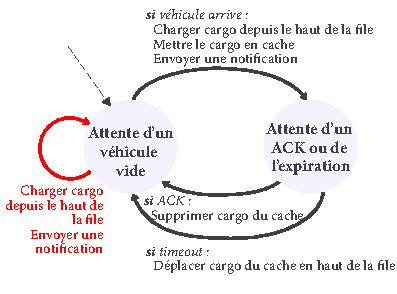
\includegraphics[height=5cm]{figures-fr/retransmissions-sender-fr.pdf} 
        \caption{Côté émetteur (point de délestage $i$).} 
        \label{fig:retransmissions-sender-fr} 
    \end{subfigure}% 
    \qquad 
    \begin{subfigure}[b]{0.45\textwidth} 
        \centering 
        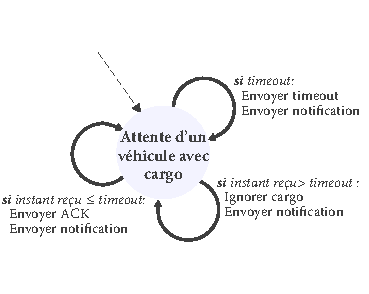
\includegraphics[height=5cm]{figures-fr/retransmissions-receiver-fr.pdf} 
        \caption{Côté récepteur (point de délestage $j$).} 
        \label{fig:retransmissions-receiver-fr} 
    \end{subfigure}% 
    \caption{Retransmissions avec SR-ARQ. Les transitions en rouge sont exclusivement pour les points de délestage intermédiaires dans le cas de la retransmission de bout-en-bout (\textbf{e2e}). Les autres transitions sont pour le point de délestage source dans le cas de retransmissions de bout-en-bout (\textbf{e2e}), et ceux source et intermédiaires dans le cas de retransmission de saut-à-saut (\textbf{hbh}).} 
    \label{fig:retransmissions-fr} 
\end{figure*} 
 
 
\paragraph{Retransmission des cargos de données.} 
Nous proposons deux types de retransmission de type SR-ARQ (\textit{Selective Repeat Automatic ReQuest} ou requête automatique avec répétition sélective) des cargos de données, en plus de la redondance des cargos arrangés avec RAID~6, puisque cette redondance ne peut pas récupérer toutes les pertes de données. D’une part, nous considérons des retransmissions de saut-à-saut (\textbf{hbh}) et d’autre part des retransmissions de bout-en-bout (\textbf{e2e}). Dans la Figure~\ref{fig:retransmissions-fr}, nous représentons le côté émetteur dans la Figure~\ref{fig:retransmissions-sender-fr} et le côté récepteur dans la Figure~\ref{fig:retransmissions-receiver-fr}. Les transitions en rouge correspondent au comportement des points de délestage intermédiaires alors que les autres transitions correspondent aux comportements du point de délestage source dans le cas de retransmissions de bout-en-bout (\textbf{e2e}) et tous les points de délestage dans le cas de retransmissions de saut-à-saut (\textbf{hbh}). Le contrôleur implémente l’un ou l’autre des deux mécanismes de retransmission au niveau des points de délestage selon leur position relative dans le transfert de données via un canal de contrôle bas-débit et longue portée  (\eg SigFox\footnote{\url{http://www.sigfox.com/}} or LoRa\footnote{\url{https://www.lora-alliance.org/}}). Chacun de ces mécanismes de retransmission repose sur un délai de temporisation (\textit{timeout} en anglais) avant retransmission correspondant au temps de trajet moyen $t(i,j)+\varepsilon$ ($\varepsilon$ constant) entre deux points de délestage $i$ et $j$. Puisque ce temps de trajet dépend des conditions de trafic routier entre les deux points de délestage, alors le contrôleur peut utiliser des services de prévision de trafic pour prévoir et réévaluer le délai de temporisation. 
 
 
Avec le premier type de retransmission de saut-à-saut (\textbf{hbh}), le contrôleur est informé des véhicules chargés quittant le point de délestage $i$. Une copie du cargo de données chargé sur le véhicule est mis en cache au niveau de $i$ jusqu’à ce que ce cargo soit transmis avec succès à $j$. Si aucun acquittement provenant de $j$ n’est reçu par le contrôleur avant l’expiration du délai de temporisation, alors le contrôleur notifie $i$ de retransmettre le cargo. Cette stratégie introduit une quantité de données additionnelles à transmettre correspondant au nombre de transmissions $R^{\textrm{hbh}}_{st}(i,\,j)$ nécessaires pour transmettre avec succès un cargo sur $(i,\,j)$~: 
\begin{equation} 
    R_{st}^{\textrm{hbh}}(i,\,j) =  \frac{1}{1-l_{st}^{\text{red}}(i,\,j)}\cdot 
\end{equation} 
 
 
Avec le second type de retransmission de bout-en-bout (\textbf{hbh}), le seul point de délestage à effectuer retransmission du cargo de donnée perdu est celui placé à la source du transfert. Une fois que le dernier point de délestage placé à la destination du transfert a reçu la donnée, celui-ci notifie au contrôleur la bonne réception du cargo de données. Ensuite, le contrôleur notifie le premier point de délestage pour enlever le cargo mis en cache lors de son chargement sur le premier véhicule l’ayant transporté. Si les points de délestage intermédiaires ne reçoivent pas le cargo attendu avant le délai de temporisation, ils notifient le contrôleur qui va demander au point de délestage source de mettre à disposition une autre copie du cargo à charger sur le prochain véhicule qui s’arrête. Cette stratégie introduit une quantité de données additionnelles à transmettre correspondant au nombre de transmissions $R^{\textrm{e2e}}_{st}(i,\,j)$ sur le lien logique $(i,\,j)$~: 
\begin{equation} 
    R^{\textrm{e2e}}_{st}(i,\,j) = \frac{(-1)^{n-(i-1)}}{\prod_{j=i}^{n-1}\big(l_{st}^{\text{red}}(j_{i},\,j_{i+1})-1\big)}\cdot 
\end{equation} 
 
 
Nous notons $O_{st}(i,\,j)$ la quantité de données additionnelles transmises par les deux mécanismes de redondance et de retransmission sur un lien logique $(i,\,j)$ pour la demande de délestage $d_{st}$. Celle-ci est exprimée par~: 
\begin{equation} 
    O_{st}(i,\,j) = \begin{dcases} 
    o_{st}^{\text{red}} \times R_{st}^{\textrm{hbh}}(i,j) & \text{\!\!\small (saut-à-saut)}\\ 
    o_{st}^{\text{red}} \times R_{st}^{\textrm{e2e}}(i,j) & \text{\!\!\small (bout-en-bout)} 
    \end{dcases} 
\end{equation} 
\noindent où $o_{st}^{\text{red}}$ est donné par l’Équation~\ref{eq:redundancy-fr}. 
 
 
Pour la modélisation, nous utiliserons la notation $o^{\text{ret}}_{st}(i,\,j)$ pour représenter la quantité de données additionnelles transmises par le mécanisme de retransmission, qu’il soit de saut-en-saut ou de bout-en-bout. De la même manière, nous utiliserons la notation $R_{st}(i,j)$ pour représenter le nombre de transmissions sur le lien logique $(i,j)$ d’un cargo de la demande de délestage $d_{st}$, indépendamment du mécanisme de retransmission utilisé. 
 
 
\paragraph{Détermination de la taille de l’arrangement en RAID~6 ($n$).} 
Pour rappel, la redondance avec RAID~6 arrange $n$ cargos de données ensemble, incluant deux cargos de données redondants. Il nous faut déterminer le nombre de cargos dans un arrangement RAID~6 de telle manière à minimiser $O_{st}$, la quantité de données additionnelles à transmettre pour une demande de délestage $d_{st}$ , en prenant en compte les cargos redondants et retransmis~: 
\[ 
    \min O_{st}=\begin{dcases} 
    \min_{n} \left\{ o_{st}^{\text{red}} \times \max_{(i,\,j)\in p}\{R_{st}^{\textrm{hbh}}(i,j)\} \right\} & \text{\!\!\small (saut-à-saut)}\\ 
    \min_{n} \left\{ o_{st}^{\text{red}} \times \max_{(i,\,j)\in p}\{R_{st}^{\textrm{e2e}}(i,j)\} \right\} & \text{\!\!\small (bout-en-bout)} 
    \end{dcases} 
\] 
 
 
 
 
\subsubsection{Modèle max-min équitable pour l’allocation des flots de véhicules} 
\label{sec:max-min-allocation-model-fr} 
 
 
À la réception d’une demande de délestage et de ses besoins en terme de performance, le contrôleur doit sélectionner les flots de véhicules sur les liens logiques selon les deux contraintes suivantes~: (\textit{i}) le nombre de véhicules disponibles doit être suffisant pour satisfaire aux besoins de la demande et (\textit{ii}) l’allocation des stockages des véhicules combinés doit être efficiente et équitable entre les transferts en compétition. Le contrôleur commence par sélectionner les chemins logiques du réseau de délestage pour chacun des transferts à délester, puis alloue des flots de données sur chacun de ces chemins tout en satisfaisant les deux contraintes. Finalement, le contrôleur configure les points de délestage le long des chemins sélectionnés avec une allocation non nulle. 
 
 
Dans la suite, $\mathcal{P}_{st}$ est l’ensemble des chemins logiques candidats entre $s$ et $t$. Chaque chemin logique $p\in\mathcal{P}_{st}$ est une séquence de liens logiques connectant des paires de points de délestage dans le réseau de délestage. Le temps de trajet $t(p)$ d’un cargo sur le chemin logique $p$ correspond au temps d’attente du cargo au niveau de chacun des points de délestage et de chacun des liens logiques traversés par le cargo. Ce temps de trajet est fonction de $R(i,j)$~: 
\begin{equation} 
    \label{eq:impl-logical-path-travel-time-fr} 
t\left(p\right) =\sum_{(i,\, j)\in p} R(i,\,j)\left[\delta_{i} + t(i,\,j)\right], 
\end{equation} 
\noindent où $\delta_i$ est le temps d’attente au point de délestage $i$. 
 
 
 
 
\paragraph{Formulation en programme linéaire.} 
Nous formulons le problème de l’allocation des ressources du réseau routier sous forme d’un modèle de programmation linéaire. Le modèle est présenté par l’Algorithme~\ref{fig:allocation-fr} et consiste à allouer une quantité $f(p)$ de données aux flots de véhicules voyageant sur les chemins logiques $p$ de $\mathcal{P}_{st}$. Nous présentons dans un premier temps les entrées de l’algorithme d’allocation et ensuite la stratégie de l’allocation des demandes de délestage. Celle-ci repose sur un problème d’allocation de multi-flots que l’on formule à l’aide d’un programme linéaire. 
 
% \removelatexerror% Nullify \@latex@error 
\begin{algorithm*}[H] 
\KwIn{Ensemble des demandes de délestage $\mathcal{D} = \{d_{st}\}$, caractérisées par $\beta_{st}$ et $\tau_{st}$} 
    \myinput{Ensembles $\{\mathcal{P}_{st}\}_{st}$ de chemins logiques entre $s$ et $t$ pour chaque demande de $\mathcal{D}$} 
    \myinput{Temps de trajet moyen $t(p)$ sur le chemin logique $p$} 
    \myinput{Capacité $c(i,\,j)$ du lien logique $(i,\,j)$} 
     
    \KwOut{Allocation résultante $A=\{f(p)\}$ des flots de données associés aux chemins logiques $p$} 
     
    \BlankLine 
    \Proc{\Alloc}{ 
        $L \gets \{\textrm{Liens logiques } (i,\,j)\}$\; 
        $\{f(p)\} \gets \textsf{Max-Min Fairness(}\mathcal{D},\,L\textsf{)}$\; 
        \Return{$\{f(p) : p\in \mathcal{P}_{st},\, (s,\,t)\in \mathcal{D}\}$} 
    } 
     
    \BlankLine 
    \Func{\MaxMin{$\mathcal{D},\,L$}}{ 
    \textit{Initialisation~:} $U\gets \mathcal{D};\;i\gets 0;\;A\gets\emptyset$\; 
    \While{$U\neq \emptyset$}{ 
    \textit{Maximiser la $i$-ème plus petite allocation~:}\; 
    \Indp  
         $\phi_{i} \gets \MCF{$\mathcal{D},\,C,\,U,\,i,\,A$}$\; 
    \Indm 
    \textit{Exécuter le test de non-blocage:}\; 
    \Indp  
 $A_{i} \gets \NBT{$U,\,A,\,\phi_{i}$}$\; 
    \Indm  
    Fixer l’allocation de chaque demande de $A_{i}$ à $\phi_{i}$\; 
    $U\gets U\backslash A_{i}$\; 
    $i\gets i+1$\; 
    } 
    \Return{$\{f(p) : p\in A\}$}\; 
    } 
     
    \BlankLine 
    \Func{\MCF{$D,\,C,\,U,\,i,\,A$}}{ 
        $\begin{array}{cc} 
\textrm{Maximiser} & \phi_{i}\end{array}$\\ 
$\begin{array}{ll} 
\textrm{Sujet à~:} & \\ 
\sum_{p}f(p)\big(\tau_{st} - t(p)\big) \geq \beta_{st} & \forall(s,\,t)\in \mathcal{D}\\ 
\phi_{i} - \sum_{p} f(p)\big(\tau_{st} - t(p)\big) \leq 0 & \forall(s,\,t)\in U\\ 
\phi_{k} - \sum_{p} f(p)\big(\tau_{st} - t(p)\big) = 0 & \forall(s,\,t)\in A_{k}, \phi_{k} \textrm{ constant},\\ 
   & k = 0,\,\dotsc,\,i-1\\ 
\sum_{s,\,t} o^{\text{red}}_{st} \sum_{p} \big[ o^{\text{ret}}_{st}(i,\,j) f(p) \big] \leq c(i,\,j) & \forall(i,\, j)\in L,\\ 
& p\textrm{ s.t. }(i,\,j)\in p\\ 
\end{array}$\; 
\Return{$\{\phi_{i}\}\cup \{f(p) : p\in \mathcal{P}_{st},\, (s,\,t)\in \mathcal{D}\}$}\; 
    } 
    \caption{Calcul des allocation des chemins logiques pour chaque demande de délestage en utilisant un modèle d’allocation max-min équitable.} 
    \label{fig:allocation-fr} 
\end{algorithm*} 


\paragraph{Entrées.} 
L’algorithme prend en entrée l’ensemble $\mathcal{D}$ de toutes les demandes de délestage. Cet ensemble inclut les demandes qui ont déjà été allouées et les nouvelles à allouer.\footnote{Il nous faut réallouer les demandes déjà allouées pour assurer de l’équité entre ces demandes et les nouvelles.} Il prend également en entrée les ensembles $\mathcal{P}_{st}$ des chemins logiques candidats entre $s$ et $t$, calculés pour chacune des demandes de $\mathcal{D}$. Pour énumérer les chemins logiques de $\mathcal{P}_{st}$, nous proposons d’utiliser l’algorithme de Yen qui calcule les $k$ plus courts chemins~\cite{yen1971finding} ou un algorithme de parcours de graphe en largeur~\cite{lee1961algorithm}. Dans nos simulations, nous réduisons l’espace de recherche en considérant les chemins ordonnés par temps de trajet pour un seul cargo de données. Enfin, l’algorithme prend en entrée le réseau de délestage et les propriétés de chacun des liens logiques (\ie capacité, temps de trajet et taux de perte).  

\paragraph{Modèle d’allocation max-min équitable.} 
Le contrôleur alloue un quantité $f(p)$ de données à chacun des chemins logiques $p$ de $\mathcal{P}_{st}$ selon la stratégie max-min équitable. Cette stratégie procède par itérations successives. La première itération alloue la quantité minimale de flots de données de manière à satisfaire les besoins d’au moins une demande (donnés par la première contrainte de la fonction \textsf{MCF}). Les itérations successives allouent les capacités restantes des liens logiques du réseau de délestage aux demandes qui peuvent recevoir une plus grande quantité de flot. Plus précisément, l’itération $i$ maximise l’allocation du flot minimal noté $\phi_{i}$ et fixe l’allocation pour les demandes qui ne peuvent pas être mieux servies (\ie soit du fait des contraintes de capacité sur les liens logiques, soit parce que les besoins des demandes ont été satisfaits par l’allocation fixée). Nous utilisons l’algorithme de test de non-blocage de l’Algorithme~\ref{fig:NBT-fr} afin de déterminer pour quels transferts de l’itération courante l’allocation peut être augmentée à l’itération suivante. 
 
 
% \removelatexerror% Nullify \@latex@error 
\begin{algorithm*}[h!] 
\KwIn{Ensemble $U$ de demandes allouées à l’itération $i$} 
\myinput{Ensemble $A$ de demandes allouées aux itérations $k<i$} 
\myinput{Allocation $\phi_{i}$ de l’itération $i$} 
\KwOut{Ensemble $A_{i}$ des flots de $U$ qui ne peuvent pas recevoir une allocation supérieure à $\phi_{i}$} 
     
    \BlankLine 
    \Func{\NBT{$U,\,A,\,\phi_{i}$}}{ 
        \textit{Les demandes qui ont été satisfaites sont allouées:}\; 
        \Indp  
            $D_{i} = \{(s,\,t) \textrm{ t.q. } \sum_{p}f(p)\big(\tau_{st} - t(p)\big) = \beta_{st} \}$\; 
            $U \gets U \backslash D_{i}; \; A_{i} = D_{i}$ \; 
        \Indm 
        \textit{Les demandes allouées plus que $\phi_{i}$ peuvent recevoir une allocation supérieure~:}\; 
        \Indp  
            $U_{i} \gets \{(s,\,t) \textrm{ t.q. } \sum_{p}f(p)\big(\tau_{st} - t(p)\big) > \phi_{i} \}$\; 
        \Indm 
        \textit{Test de l’allocation des demandes restantes~:}\; 
        \ForEach{demande $(s,\,t)\in U\backslash (A_{i}\cup U_{i})$}{ 
            $\begin{array}{@{}ll@{}} 
            \textit{Résoudre le programme linéaire suivant~:} & \\ 
    \textrm{Maximiser} & \sum_{p\in\mathcal{P}_{st}} f(p)\\ 
    \textrm{Sujet à:} & \\ 
    \sum_{p}f(p)\big(\tau_{st} - t(p)\big) \geq \beta_{st} & \forall(s,\,t)\in D\\ 
    \phi_{k} - \sum_{p} f(p)\big(\tau_{st} - t(p)\big) = 0 & \forall(s,\,t)\in A_{k}, \phi_{k} \textrm{ constant}, \\ 
       & k = 0,\,\dotsc,\,i-1\\ 
    \sum_{s,\,t} o^{\text{red}}_{st} \sum_{p} \big[ o^{\text{ret}}_{st}(i,\,j) f(p) \big] \leq c(i,\,j) & \forall(i,\, j)\in C,\\ 
    & p\textrm{ s.t. }(i,\,j)\in p\\ 
    \end{array}$\; 
     
            \lIf{$\sum_{p\in\mathcal{P}_{st}} f(p) \leq \phi_{i}$}{ 
                $A_{i} \gets A_{i}\cup \{(s,\,t)\}$\; 
            } 
            \lElse{$U_{i}\gets U_{i} \cup \{(s,\,t)\}$}\; 
        } 
         
        \Return{$A_{i}$}\; 
    } 
     
    \caption{Test de non-blocage pour le modèle d’allocation max-min équitable.} 
    \label{fig:NBT-fr} 
\end{algorithm*} 
 
 
La fonction \textsf{MCF} (\textit{Multi-Commodity Flow}) est au cœur de l’algorithme max-min équitable et est définie dans l’Algorithme~\ref{fig:allocation-fr}. Celle-ci calcule une allocation de multi-flots. La première contrainte fait correspondre la quantité de données qui peut être délestée pendant le temps imparti $\tau_{st}$ avec la quantité de données à transférer $\beta_{st}$. La contrainte suivante garantie que les demandes appartenant aux ensembles $A_{k},\,k\in [0,\,i-1]$ sont fixées à l’allocation qu’elles ont reçue à l’itération $k$. L’objectif de la fonction \textsf{MCF} est de maximiser l’allocation minimum $\phi_{i}$ telle que toutes les demandes soient satisfaites. Cet objectif est garanti par la troisième contrainte du problème linéaire. Enfin, la dernière contrainte limite la quantité cumulée des allocations sur les chemins logiques à la capacité maximale des liens logiques. Cette contrainte prend en compte les données additionnelles transmises avec les mécanismes de redondance et de retransmission. 
 
 
Une fois que l’allocation $\phi_i$ a été fixée par la fonction \textsf{MCF} à l’itération $i$, l’algorithme max-min équitable détermine quelles demandes peuvent être augmentées par rapport à leur allocation courante en utilisant le test de non-blocage de l’Algorithme~\ref{fig:NBT-fr}. Le test de non-blocage est adapté de l’algorithme proposé par Pi\'{o}ro \etal~\cite{pioro2003efficient}. Ce test compare le débit maximal des flots alloués par une allocation multi-flots par rapport à celle qui résulte de l’allocation minimale $\phi_{i}$. Si l’allocation multi-flots augmente la quantité maximale de données allouée à une demande, celle-ci est non-bloquante et peut être fixée dans l’une des prochaines itérations de l’algorithme max-min équitable. Sinon, l’allocation de la demande ne peut pas être augmentée et est fixée à $\phi_{i}$. 
 
 
Cette formulation d’allocation multi-flots reste valide pour des flots continus de données (par exemple, des demandes avec un débit constant). Dans ce cas, il nous suffit d’adapter la première contrainte de la fonction \textsf{MCF} pour satisfaire aux besoins de la demande en l’exprimant en fonction du débit à atteindre. 

 
\subsubsection{Ordonnancement des données} 
Afin d’ordonnancer les données, chaque point de délestage utilise des ``tables de flots'' configurées par le contrôleur suite à l’allocation des flots de véhicules pour faire correspondre les données disponibles localement avec les véhicules à l’arrêt et décider d’une action à prendre (\ie charger un cargo de données sur le véhicule, décharger un cargo ou échanger des cargos). Une entrée de la table de flot contient le prochain saut (\ie point de délestage) correspondant au chemin logique alloué pour une demande de délestage donnée. La direction du véhicule à l’arrêt est prédite par le contrôleur et mise en correspondance avec le prochain saut de chacune des entrées de la table de flot (pour chacune des entrées dont les cargos de données associés sont disponibles localement au point de délestage). Si aucune des entrées ne correspond à la destination du véhicule, alors le cargo transporté par le véhicule est déchargé et mis en transbordement au niveau du point de délestage pour être transporté par les véhicules suivants. Dans le cas où plusieurs entrées correspondent à la direction du véhicule, le point de délestage sélectionne l’entrée selon la politique d’ordonnancement décrite ci-après. Si le véhicule transporte un cargo de données, le point de délestage vérifie qu’elles n’appartiennent pas déjà au flot sélectionné. Si tel est le cas, aucune action n’est entreprise et le véhicule continue sa route. Sinon, le cargo est déchargé du véhicule. Dans le cas d’un véhicule vide, le cargo le plus ancien de données correspondant aux entrées sélectionnées est chargé sur le véhicule.  
 
 
Dans le cas où plusieurs entrées de la table de flot du point de délestage $i$ correspondent à la direction du véhicule à l’arrêt, $i$ sélectionne l’entrée selon une politique d’ordonnancement de type \textit{weigthed fair queuing}, dont les poids sont configurés par le contrôleur suivant le résultat de l’allocation des flots de véhicules. Nous notons $f(d_kp_l)$ le flot de données sur le chemin logique $p_l$ alloué au transfert résultant de la demande de délestage $d_k$. Le contrôleur assigne un poids $w(d_kp_l)$ à chacun des transferts alloués sur le chemin logique $P = \{d_kp_l | \forall d_k\in D,\, p_l\in \mathcal{P}^{d_k},\, (i,\,j) \in p_l\}$, où $P$ est l’ensemble des chemins logiques traversant à la fois le point de délestage $i$ et le lien logique $(i,\,j)$ connectant $i$ au prochain saut $j$. Le contrôleur calcule le poids $w(d_kp_l)$ en normalisant le débit du flot $f(d_kp_l)$ par rapport au débit total des flots de $P$~: 
\begin{equation} 
    w(d_kp_l) = \frac{f(d_kp_l)}{\sum_{p\in P} f(p)}\cdot 
\end{equation} 
 
 
Nous utilisons les poids de l’algorithme d’ordonnancement pour déterminer la priorité des transferts de données à assigner aux cargos de données pour en charger un dans le véhicule à l’arrêt, dans le cas où plusieurs allocations de transferts traversent le même point de délestage. Dans nos simulations, nous considérons une politique d’ordonnancement de type \textit{weigthed fair queuing} qui utilise ces poids afin de sélectionner de manière aléatoire un cargo de données à charger dans le véhicule à l’arrêt~\cite{shreedhar1996efficient}. 
 
 
 
 
\subsection{Évaluation sur les routes françaises} 
\label{sec:evaluation-fr} 
 
 
\paragraph{Jeu de données.} 
Pour évaluer le délestage des données, nous utilisons un jeu de données routières de la DTITM (Direction Technique Infrastructures de Transports et Matériaux). Ces données comportent les trafics moyens journaliers annuels (TMJA) de 2011 sur 20 000 km d’autoroutes et routes nationales en France.\footnote{Données de la DGITM/DIT~--~SETRA~--~IGN (\url{http://tinyurl.com/otfbewv})} 
 
 
Pour les besoins de cette évaluation, nous avons simulé un plan de déploiement de ces stations sur le territoire français à l’aide d’un algorithme d’allocation de facilités. Les stations sont allouées pour maximiser les demandes venant des villes, pondérées par leur taille, de telles sorte qu’elles soient toutes placées au plus à 150~km l’une de l’autre (représenté sur la Figure~\ref{fig:France-location-allocation-fr}). En effet, l’autonomie moyenne d’un véhicule étant de 300~km, cette allocation permet à un véhicule de rejoindre la prochaine station sur sa route ou de rejoindre la précédente. L’allocation donne 38 stations de chargement réparties sur le réseau routier français, comme montré sur les Figures~\ref{fig:France-location-allocation-fr} et~\ref{fig:France-overlay-wo-capacity-fr}.  
 
 
\begin{figure}[ht] 
    \centering 
    \begin{subfigure}[t]{0.47\columnwidth} 
            \centering 
            % \raisebox{.2\textwidth}{ 
            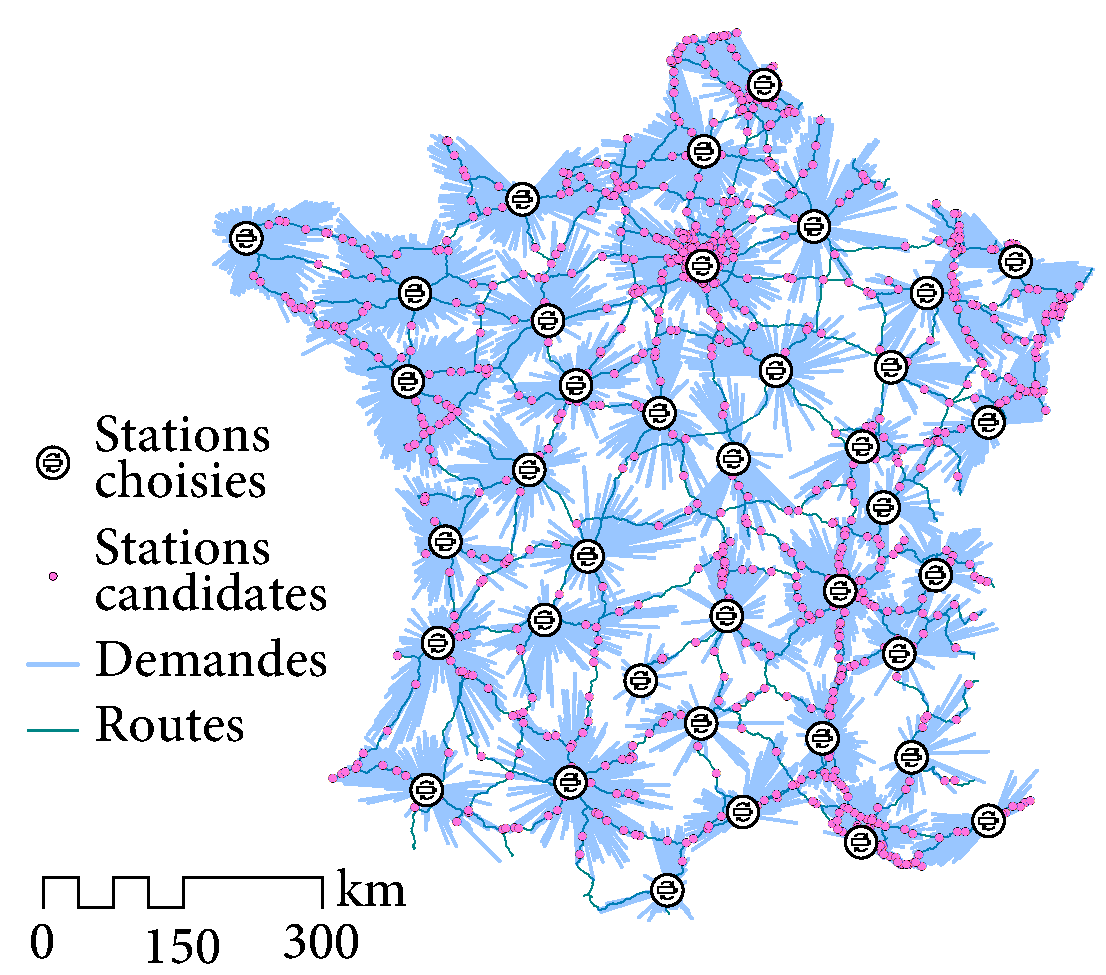
\includegraphics[width=0.98\textwidth]{figures-fr/France-allocation-charging-stations-fr.pdf} 
            % } 
            \caption{Allocation des stations de chargement de batteries électriques sur le réseau routier français. Les gros points sont les stations choisies et les lignes représentent les demandes allouées aux stations choisies.} 
            \label{fig:France-location-allocation-fr} 
    \end{subfigure}% 
    \quad %add desired spacing between images, e. g. ~, \quad, \qquad etc. 
      %(or a blank line to force the subfigure onto a new line) 
    \begin{subfigure}[t]{0.5\columnwidth} 
            \centering 
            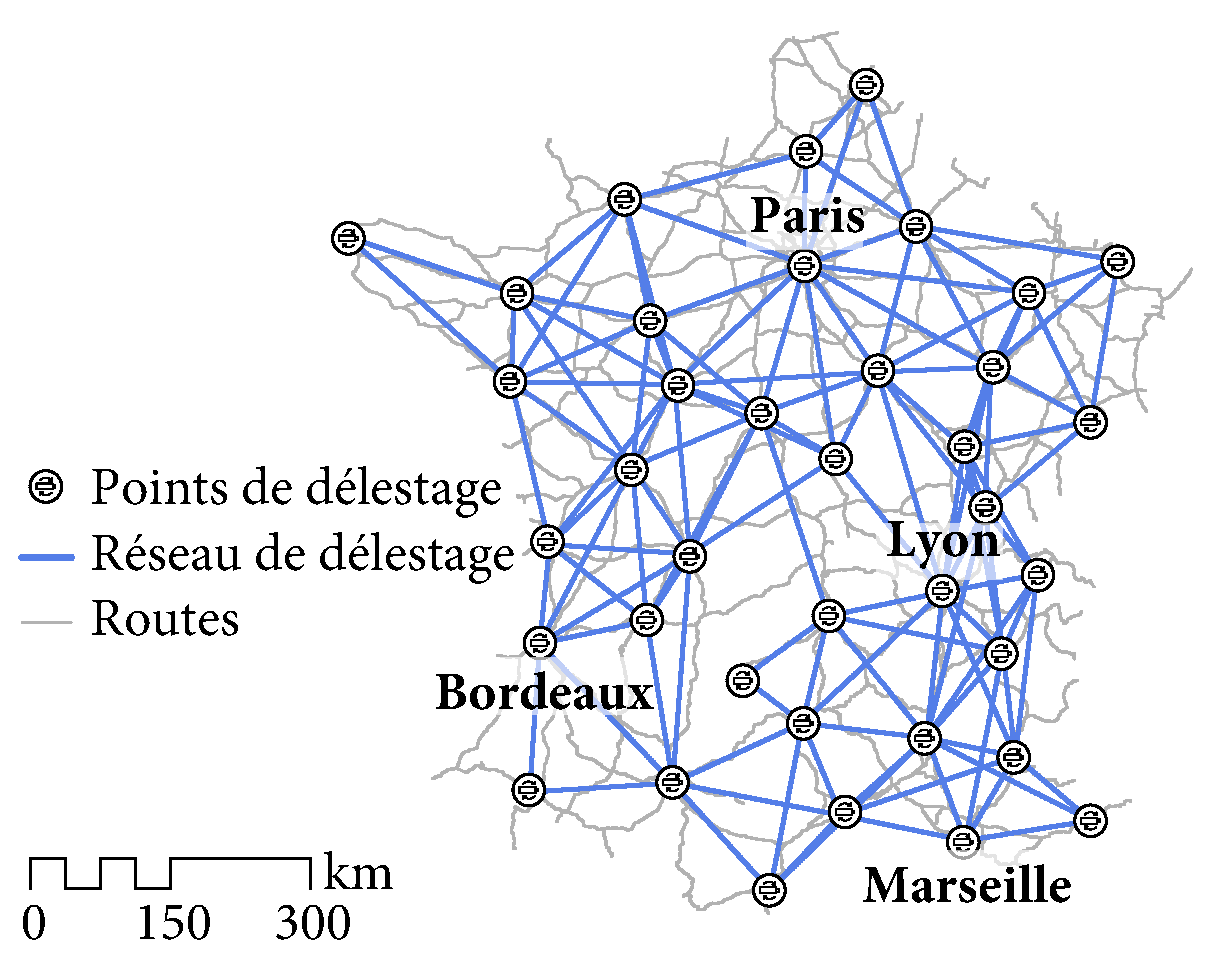
\includegraphics[width=\textwidth]{figures-fr/France-overlay-wo-capacity-fr.pdf} 
            \caption{Le réseau de délestage construit à partir du réseau routier français. Les points de délestage sont ceux représentés sur la Figure~\ref{fig:France-location-allocation-fr}.} 
            \label{fig:France-overlay-wo-capacity-fr} 
    \end{subfigure} 
    \caption{Résultat de l’allocation de facilité et réseau de délestage. Les gros points sont les stations de chargement choisies.} 
\end{figure} 
 
 
 
 
\paragraph{Création du réseau de délestage.} 
Le réseau de délestage est créé en considérant les stations de chargement précédemment déployées. Le but est de caractériser ses liens logiques par des quantités réseau en déterminant les volumes de trafic routier entre chaque paire de points de délestage. Ces volumes sont donnés par des matrices origine-destination connectant les points de délestage. Cependant, ces matrices sont rarement disponibles (voire pas du tout disponibles) pour des réseaux routiers à large-échelle. Nous les déduisons de jeux de données disponibles publiquement contenant les valeurs de Trafic Moyen Journalier Annuel (TMJA) pour chacun des tronçons de route du réseau routier français. Ainsi, en utilisant des techniques bien connues de prévision de trafic routier issues des recherches en transportation, nous sommes à même d’en déduire les matrices origine-destination nécessaire à notre caractérisation du réseau de délestage. Nous procédons aux trois étapes suivantes~: 
 
 
\begin{enumerate} 
    \item \textit{Détermination des routes.}  
    La première étape consiste à sélectionner un sous-ensemble de routes alternatives (à la route la plus courte) du réseau routier connectant chaque paire de points de délestage. Cette étape consiste à sélectionner les $k$ routes les plus courtes en terme de temps de trajet. Les routes sont sélectionnées de telle manière qu’elles ne partagent qu’un faible degré de similarité entre elles en terme de tronçons de route en commun. Nous implémentons cette étape en utilisant les algorithmes proposés par Abraham \etal~\cite{abraham2013alternative}. 

    \item \textit{Assignement des routes.}  
    La seconde étape consiste à pondérer les routes sélectionnées en utilisant le modèle d’assignement des routes C-logit~\cite{cascetta1996modified}. Les valeurs de poids sont déterminées selon le temps de trajet et la distance des routes. Ces poids reflètent la capacité d’une route à attirer du trafic, avec une grande valeur de pondération, la route attire plus de trafic routier par rapport à une route avec une petite valeur de pondération. Les poids sont ensuite utilisés avec les TMJA des tronçons pour estimer les volumes de trafic entre les points de délestage. 
 
    \item \textit{Estimation de la matrice origine-destination.} 
    Dans cette troisième étape, nous utilisons un modèle de maximisation d’entropie proposé par Zuylen et Willumsen pour calculer la matrice d’origine-destination entre chaque paire de points de délestage du réseau de délestage~\cite{van1980most}. Ce modèle détermine la distribution de trafic la plus probable sur les routes déterminées durant la première étape et est sujet à deux contraintes~: (\textit{i}) la capacité des tronçons de route pour les routes sélectionnées données par les TMJA et (\textit{ii}) les poids déterminés par le modèle d’assignement des routes C-logit présenté lors de la deuxième étape. Nous utilisons un jeu de données donnant les TMJA des tronçons de route de France afin d’en inférer les matrices origine-destination. 
 
\end{enumerate} 
 
\begin{wrapfigure}[14]{o}[0.7\marginparwidth]{7.5cm}
    \vspace{-15pt}
    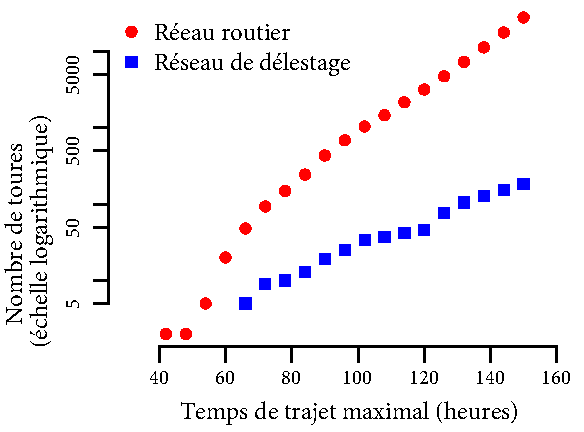
\includegraphics[width=7.2cm]{figures-fr/pathcount-fr.pdf}
    \caption{Nombre total de chemins dans le réseau routier français et du réseau de délestage en fonction du temps de trajet maximal.}
    \label{fig:pathcount-fr}
\end{wrapfigure}
Finalement, à partir de la matrice origine-destination entre chaque paire de point de délestage, nous déterminons les attributs de chaque lien logique $(i,\,j)$ du réseau de délestage. Pour rappel, ces attributs sont la capacité, le temps de trajet et le taux de perte.  
La Figure~\ref{fig:pathcount-fr} montre le nombre de chemins en fonction du temps de trajet. Dans chacun des deux cas, le nombre de chemins possibles augmente de manière exponentielle avec le temps de trajet. Cependant, le nombre de chemins est beaucoup plus grand pour le réseau routier, comparé au nombre de chemins du réseau de délestage. De plus, la différence du nombre de chemins possibles augmente de manière exponentielle également. C’est cette différence qui consititue le facteur principal de complexité quand il s'agit de résoudre le problème de l'allocation de flots de véhicules. Ainsi, ce réseau de délestage permet de simplifier l’infrastructure routière tout en préservant les propriétés des chemins acceptables avant agrégation. 
 
\paragraph{Modèle d’allocation max-min équitable sur le réseau routier de France.} 
Nous évaluons les performances des transferts résultant de l’allocation de \textit{trois} demandes de délestage. Celles-ci sont représentées sur la Figure~\ref{fig:france-demand-allocation-haulage-fr}~:  
(\textit{i}) $d_A$ de Paris à Lyon avec un taux d’arrivées Poissoniennes $\lambda_A$,  
(\textit{ii}) $d_B$ de Paris à Bordeaux avec un taux d’arrivées Poissoniennes $\lambda_B$, et  
(\textit{iii}) $d_C$ de Paris à Marseille avec un taux d’arrivées Poissoniennes $\lambda_C$. Il faut noter que les chemins suivis par les transferts résultant des demandes $d_A$ et $d_C$ partagent le même lien logique dans le réseau de délestage. De fait, $d_A$ et $d_C$ vont être en compétition pour prendre la capacité de ces liens logiques.  
 
\begin{wrapfigure}[14]{o}[0.7\marginparwidth]{8cm} 
    \centering 
    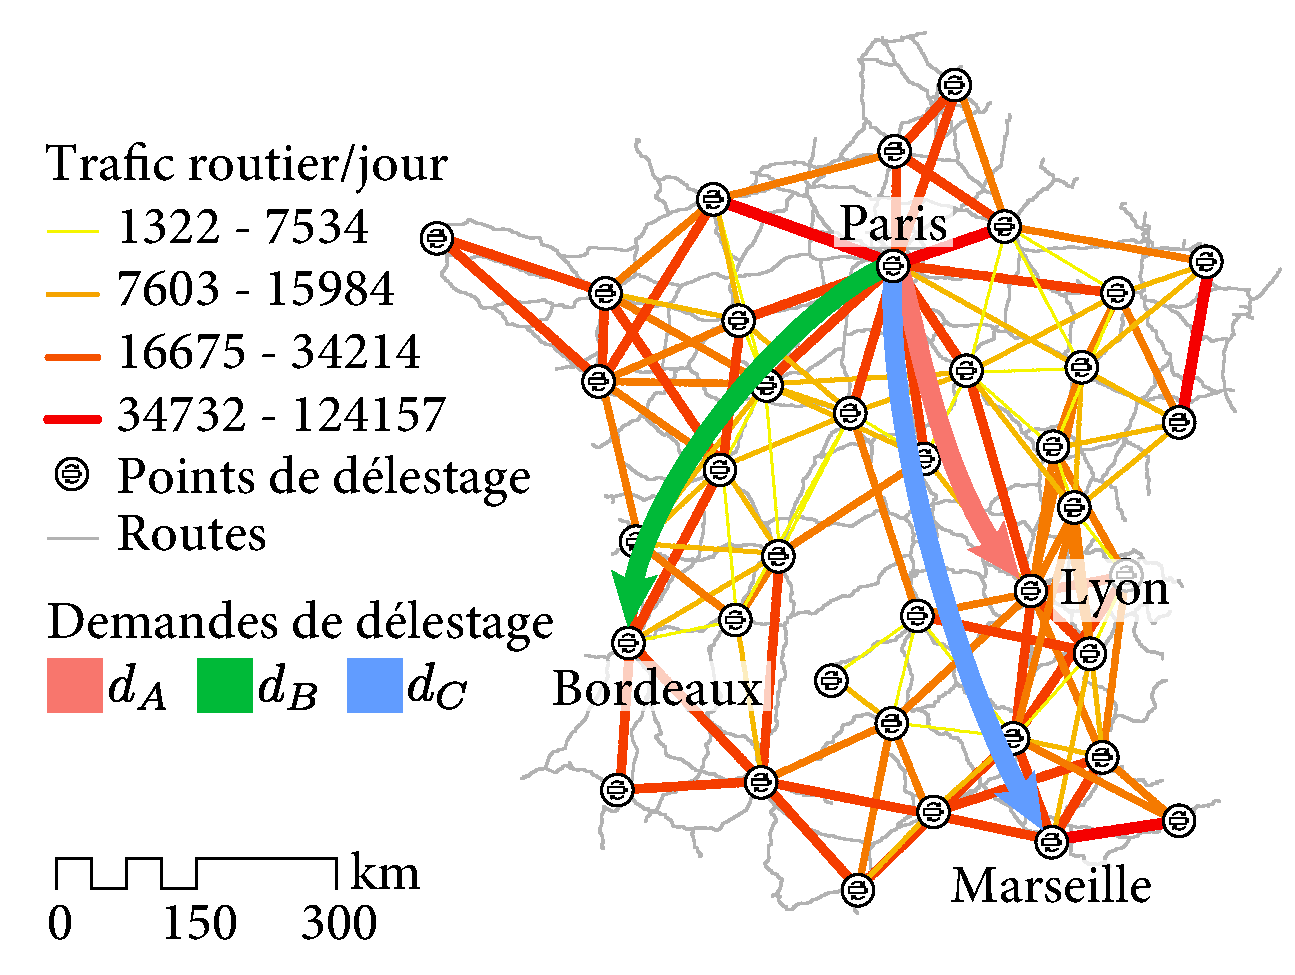
\includegraphics[width=7.5cm]{figures-fr/France-overlay-haulage-fr.pdf} 
    \caption{Représentation schématiques des trois demandes de délestage $d_A$, $d_B$ et $d_C$.} 
    \label{fig:france-demand-allocation-haulage-fr} 
\end{wrapfigure} 
Nous choisissons des paramètres volontairement pessimistes: nous supposons uniquement 10\% du parc automobile français équipé de capacités de stockage égal à 1~Téraoctet sur chaque véhicule. Nous supposons que les stations de chargement ont une capacité qui correspond à la demande pour charger des véhicules électriques, ce qui donne un temps d’attente nul avant d’être servi. Le temps d’attente est donc réduit au temps de service, qui correspond au temps de charge de la batterie électrique. Nous supposons le taux d’erreur sur les liens logiques du réseau de délestage égal pour chacun des liens, indépendamment de leur longueur ou volume de trafic. 
 
 
Nous effectuons les simulations avec le simulateur de trafic SUMO (\textit{Simulation of Urban MObility}), duquel nous récupérons et traitons les évènements via l’API TraCI~\cite{behrisch2011sumo}. La durée de chaque simulation est de 300~000~secondes (3,5~jours), incluant 43,200~secondes (12~heures) d’initialisation (\textit{warmup} en anglais) pour remplir les stockages des points de délestage. 
 
\begin{wrapfigure}[12]{o}[0.7\marginparwidth]{6cm}
    \vspace{-15pt}
    \centering
    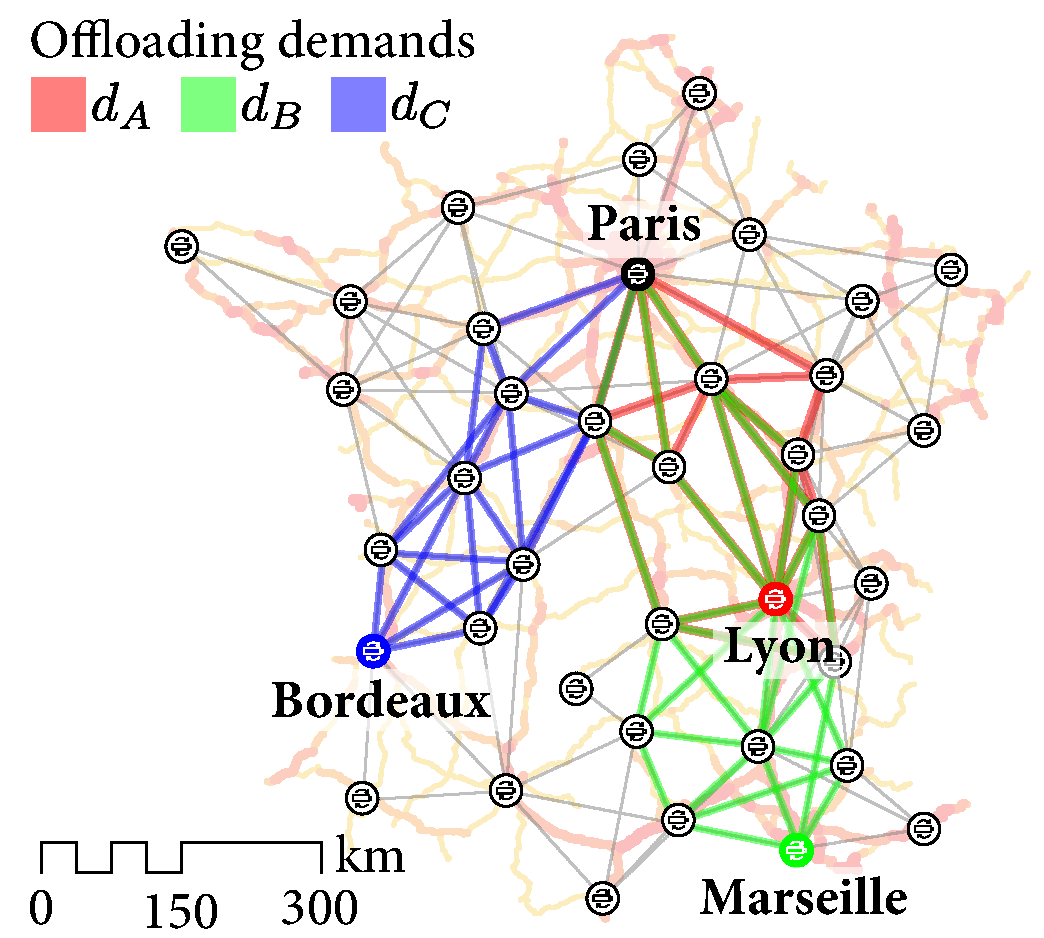
\includegraphics[width=5.4cm]{figures-fr/France-AADT-overlay-layers-fr.pdf}
    \caption{Chemins logiques alloués aux demandes $d_A$, $d_B$ et $d_C$.}
    \label{fig:allocation-subpaths-offloading-overlay-fr}
\end{wrapfigure}
\paragraph{Débit maximum atteignable.} 
Nous évaluons le débit maximum atteint par chacun des transferts $d_A$, $d_B$ et $d_C$ résultant de la stratégie d’allocation max-min équitable présentée dans la Section~\ref{sec:max-min-allocation-model-fr}. Nous considérons également une autre stratégie sans contrôleur identique à celle présentée dans la section~\ref{sec:scenario-simple-fr} qui sélectionne les cargos de données à charger dans les véhicules à l’arrêt selon la politique d’ordonnancement \textit{Round-Robin}. Nous considérons un trafic ininterrompu de données généré par une seule source située à Paris pour chacun des transferts (\ie $\lambda_A=\lambda_B=\lambda_C=\infty$). Nous évaluons le débit maximum atteint pour chaque stratégie et chaque mécanisme de retransmission (\ie saut-à-saut et bout-en-bout) présentés dans la Section~\ref{sec:fiabilite-fr}. Celui- est représenté sur la Figure~\ref{fig:french-net-throughput-leakage-fr} en fonction du taux d’erreur sur les liens logiques. Le débit est exprimé en terme de nombre de cargos de données livrés par seconde. 
 
 
\begin{figure}[h!] 
    \centering 
    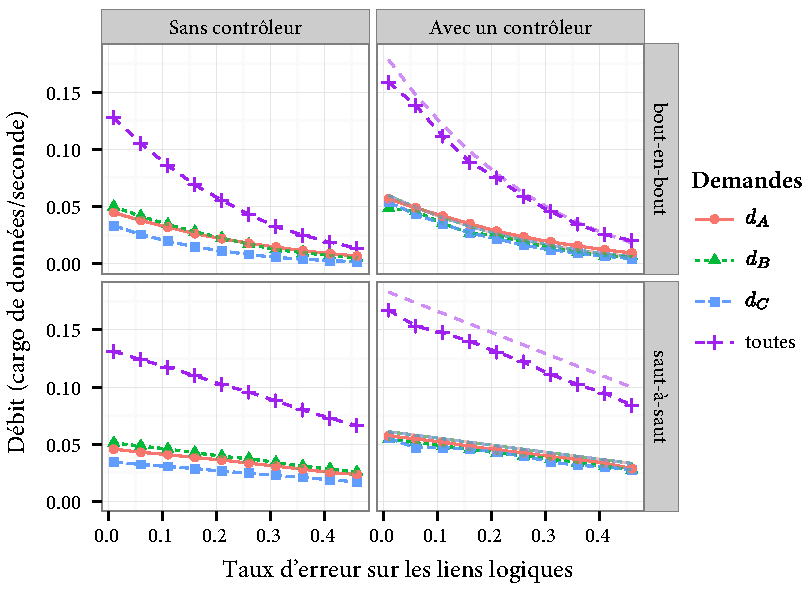
\includegraphics[width=0.65\textwidth]{figures-fr/plot-france-rate-throughput-m-10-wo-MCF-fr.pdf} 
    \caption{Débit maximum pour les demandes de délestage $d_A$, $d_B$ et $d_C$ (représentées dans la Figure~\ref{fig:france-demand-allocation-haulage-fr}) en fonction du taux d’erreur sur les liens logiques (supposé égal pour chacun des liens logiques).} 
    \label{fig:french-net-throughput-leakage-fr} 
\end{figure} 
 
Dans un premier temps, nous examinons le débit résultant de la stratégie sans contrôleur. Cette stratégie ne garantie pas un débit réparti équitablement entre les transferts résultant des trois demandes. Le débit maximum pour la demande $d_C$ est inférieur comparé à ceux des deux demandes $d_A$ et $d_B$. Comme montré sur la Figure~\ref{fig:allocation-subpaths-offloading-overlay-fr} (dans le cas avec contrôleur), les transferts de données résultants des demandes $d_A$ et $d_C$ sont en compétition pour les mêmes ressources, puisqu’elles partagent toutes deux des liens logiques. La stratégie d’ordonnancement sans contrôleur alloue les flots de véhicules voyageant le long de ces liens vers les destinations respectives de $d_A$ et $d_C$ sans prendre en compte le fait que la destination de $d_C$ est plus éloignée que celle de $d_A$. Ainsi, la stratégie favorise $d_A$ au dépend de la demande $d_C$. Le transfert résultant de la demande $d_B$, quant à lui, n’est pas affecté puisque les flots de véhicules alloués à $d_B$ voyagent le long de chemins logiques différents par rapport à $d_A$ et $d_C$. Nous pouvons aussi noter que le débit maximum pour les transferts $d_A$ et $d_B$ ont des valeurs similaires puisque leur destinations sont équidistantes de leur source.
 
Dans un second temps, nous examinons la stratégie avec un contrôleur. Nous constatons que cette stratégie donne de meilleurs débits cumulés que la stratégie sans contrôleur. C’est la conséquence directe de la conception des deux stratégies d’ordonnancement. La stratégie avec contrôleur utilise une allocation max-min équitable qui alloue les flots de véhicules de façon à maximiser les flots de données alloués et à garantir l’équité entre les transferts alloués en concurrence. L'allocation alloue les chemins logiques pour chacune des demandes comme représenté sur la Figure~\ref{fig:allocation-subpaths-offloading-overlay-fr}. La meilleure performance de cette stratégie confirme le besoin d'un contrôleur, comme nous l’avions montré dans la Section~\ref{sec:scenario-simple-fr}. Les résultats confirment également que la stratégie avec un contrôleur garantie une allocation équitable entre les transferts résultants des trois demandes de délestage.  

Enfin, le mécanisme de retransmission de type saut-à-saut donne de meilleurs résultats par rapport à celui de type de bout-en-bout. Le premier mécanisme recouvre les erreurs plus rapidement que le second, qui demande à la source de retransmettre le cargo de données. Celui-ci doit alors parcourir à nouveau tout le chemin déjà parcouru par le cargo perdu. En contrepartie, la stratégie de type bout-en-bout nécessite moins de stockage localement au niveau des points de délestage pour mettre en cache les cargos chargés dans les véhicules (les cargos mis en cache sont utilisés par la stratégie de type saut-à-saut pour récupérer les cargos perdus).  
 
Pour des cargos de taille 1~Téraoctet, l’allocation qui résulte de la stratégie avec un contrôleur donne un débit cumulé de 114~Gigabits par seconde en utilisant le système de retransmission de type saut-à-saut et avec un taux d’erreur de 30\%. Cela correspond à une moyenne de 38~Gigabits par seconde pour chacun des trois transferts. 
 
\section{Extension à des services véhiculaires de type ``cloud''} 

Dans ce chapitre, nous étendons le concept de point de délestage selon deux directions afin d’en faire une base pour développer des services véhiculaires de type ``cloud''. 
 
Dans une première section, nous exploitons les capacités de stockage des points de délestage pour concevoir un système distribué de stockage et de partage de fichiers générés par des utilisateurs mobiles. Les points de délestage jouent le rôle de dépôts où les utilisateurs mobile y déposent et récupèrent des fichiers. Pour augmenter les chances de trouver le fichier recherché en un temps imparti, les dépôts distribuent les fichiers entre eux en utilisant les mouvements existants des utilisateurs les visitant.
 
Dans une seconde partie, nous dématérialisons les points de délestage en zones prédéfinies où les véhicules sont en contact fréquemment et suffisamment longtemps pour pouvoir transférer des fichiers de grosse taille. Nous utilisons ces zones dans le contexte de virtualisation de réseaux véhiculaires où les ressources des véhicules (\ie calcul, stockage et communications) sont partagées en utilisant des machines virtuelles. Les machines virtuelles sont allouées à un fournisseur de service qui utilise les mouvements des véhicules hébergeant les machines virtuelles pour déployer des services géo-distribués à large-échelle (par exemple, des plateformes de capteurs). En particulier, nous nous intéressons à la capacité des contacts entre les véhicules dans ces zones prédéfinies pour effectuer les migrations de machines virtuelles nécessaires en cas de changements de topologie ou de réallocation des ressources des véhicules.
 
Dans chacune de ces deux extensions, nous proposons un placement optimisé des points de délestage selon les besoins spécifiques aux services à mettre en place. Ainsi, nous utilisons les concepts vus dans la première partie de cette thèse avec le réseau de délestage pour obtenir une vue logique des mouvements des véhicules entre les points de délestage. 
 
 
\subsection{Système véhiculaire de stockage et partage de fichiers} 
\label{sec:system-cloud-storage-fr} 
 
 
Dans cette section, nous présentons un système de stockage et de partage de fichiers pour utilisateurs mobiles. Ce système repose sur un ensemble de facilités dédiées équipées de stockage pré-positionnées à des endroits stratégiques qui jouent le rôle de dépôts pour fichiers. Les utilisateurs mobiles stockent leurs fichiers qu’ils souhaitent archiver ou partager avec d’autres utilisateurs, puisque ces fichiers peuvent être récupérés plus tard par leur propriétaire ou par d’autres utilisateurs depuis n’importe quel dépôt du système. Les utilisateurs émettent des requêtes pour stocker et récupérer des fichiers dans les dépôts du système. Afin de limiter le nombre de requêtes actives simultanément, celles-ci disposent d’un temps imparti avant lequel elles doivent être satisfaites. Au bout du temps imparti, la requête expire et est considérée comme étant non satisfaite. 
 
 
Le système ne considère aucune connexion réseau disponible entre les dépôts, rendant impossible de récupérer un fichier depuis un dépôt autre que celui où le fichier avait été stocké en premier lieu. Afin de résoudre ce problème, le système exploite les mouvements des utilisateurs entre les dépôts pour partager les copies des fichiers stockés et ainsi les répliquer au sein des dépôts du système. Notons qu’exploiter la mobilité des utilisateurs limite la dépendance vis-à-vis des réseaux de données traditionnels qui pourraient être utilisés pour connecter les dépôts entre eux. Afin d’augmenter les chances de répliquer les fichiers entre les dépôts, plusieurs copies des fichiers sont transportés par différents utilisateurs. 
 
 
Le problème qui nous intéresse dans ce travail est de placer un nombre cible de dépôts en fonction du temps imparti pour satisfaire les requêtes des utilisateurs. De ce fait, le placement est contraint par les deux objectifs suivants~: 
\begin{enumerate} 
    \item Déterminer les emplacements des dépôts pour qu’ils servent un nombre maximal de requêtes avant qu’elles n’expirent. 
 
 
    \item Connecter les dépôts entre eux par les mouvements des utilisateurs afin de répliquer les fichiers entre dépôts. 
\end{enumerate} 
 
 
\subsubsection{Placement des dépôts} 
 
\begin{wrapfigure}[13]{o}[0.3\marginparwidth]{7.2cm} 
    \vspace{-10pt} 
    \centering 
    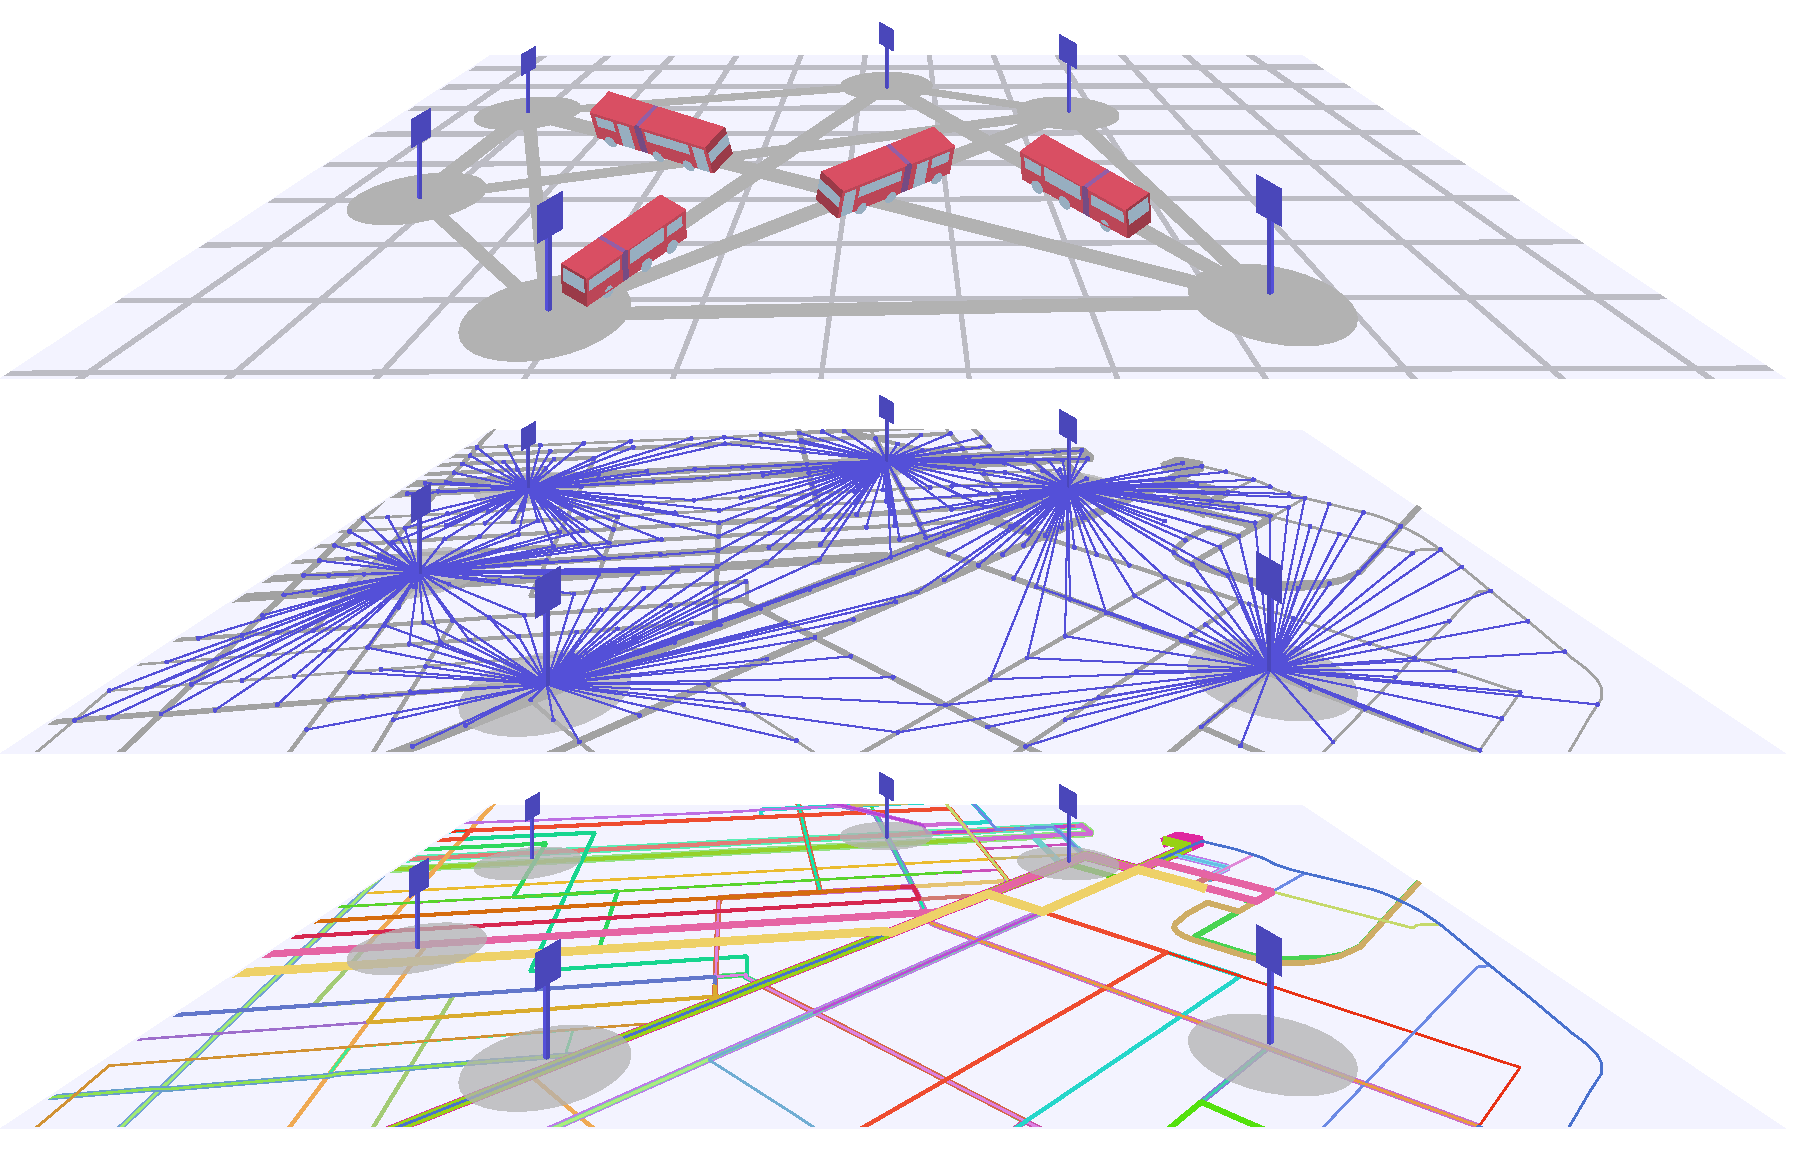
\includegraphics[width=7cm]{figures-fr/bus-distribution-system-fr.pdf} 
    \caption{Différentes couches illustrant les différentes étapes de l’algorithme de placement des dépôts dans le cas d’un système de bus.} 
    \label{fig:placement-alg-fr} 
%\end{figure} 
\end{wrapfigure} 
Les différentes étapes de l’algorithme du placement des dépôts sont illustrées avec la Figure~\ref{fig:placement-alg-fr} dans le cas d’un système de bus. La couche inférieure montre les trajectoires de bus du quartier des affaires de San Francisco aux États-Unis et le sous-ensemble d’arrêts de bus jouant le rôle de dépôts de fichiers. Chaque ligne de bus est représentée par une couleur et une épaisseur indiquant la fréquence à laquelle les bus voyagent sur cette ligne. La couche du milieu montre les demandes discrétisées représentant les requêtes générées par les passagers de bus. De plus, cette couche montre comment les demandes discrétisées sont allouées aux différents dépôts selon leur distance respective aux dépôts. Enfin, la couche supérieure montre un graphe logique dont les nœuds correspondent aux dépôts et les liens correspondent aux flots de bus voyageant entre les dépôts. De la même manière que pour la couche inférieure, l’épaisseur des liens correspond à la fréquence des routes des bus. 

La formulation du placement des dépôts est dérivée du problème de couverture par ensembles, et en particulier le problème de couverture maximale~\cite{church1974maximal}. Étant donné un ensemble d’emplacements candidats pour des dépôts, le problème de placement consiste à sélectionner les dépôts tels que leur couverture maximise le taux de succès des requêtes générées par les utilisateurs. Ce problème a été montré NP-Complet~\cite{megiddo1983maximum}, donc il nous faut adapter des heuristiques connues pour le résoudre. De ce fait, nous considérons l’heuristique gloutonne (\textit{greedy} en anglais) d’ajouts avec substitutions (GAS)~\cite{church1974maximal} qui détermine les emplacements optimaux pour chaque itération de l’algorithme.  
 
 
\subsubsection{Simulation avec des traces réalistes} 
\label{sec:simulation-traces-reelles-fr} 
 
 
Afin d’évaluer l’algorithme de placement de dépôts, nous effectuons dans un premier temps un déploiement d’un nombre prédéfini de dépôts en considérant les arrêts et routes des bus opérés par MUNI à San Francisco aux États-Unis.\footnote{\url{https://www.sfmta.com/}}\index{Muni|see {San Francisco municipal transportation agency}} Nous recréons les mouvements des bus et ensuite sélectionnons les arrêts où déployer les dépôts. 
 
 
Nous faisons les hypothèses suivantes. Les utilisateurs mobiles sont des passagers des bus. Les dépôts sont équipés d’interfaces réseau de type IEEE 802.11 avec une portée de 250~m. Pour un souci de simplicité, nous ignorons les interférences et supposons que la capacité de ces interfaces est suffisante pour transférer l’ensemble des fichiers (quel qu’il soit) entre les dépôts et les passagers des bus. Les bus s’arrêtent aux arrêts pour une durée aléatoire comprise entre 10~secondes et 30~secondes. Par ailleurs, nous ne faisons aucune supposition sur la popularité géographique des fichiers~: une requête est générée par un utilisateur  en moyenne chaque 10~minutes de temps simulé selon une distribution Poissonienne. Nous considérons deux types de requêtes avec les proportions suivantes~: 10\% des requêtes sont des requêtes pour stocker un fichier et 90\% des requêtes récupèrent un fichier. La durée de simulation est de 20~000~secondes. 
 
 
\begin{figure}[t!] 
    \begin{subfigure}[t]{0.4\textwidth} 
        \centering 
        \includegraphics[width=0.9\linewidth]{figures-fr/sf-muni-placement-fr.pdf} 
        \caption{Placement des dépôts. Les variations de couleurs des demandes et des candidats représentent des points chauds (\textit{hotspot} en anglais), correspondant à des emplacements signifiants spatialement, calculé en utilisant les $p$-valeurs des fréquences moyennes de visites de l’analyse spatiale Getis Ord-G~\cite{getis1992analysis}.} 
        \label{fig:sf-muni-placement-fr} 
    \end{subfigure} 
    \qquad 
    \begin{subfigure}[t]{0.55\textwidth} 
        \centering 
        \includegraphics[width=.9\linewidth]{figures-fr/origin-destination-matrix-fr.pdf} 
        \caption{Matrice origine-destination des dépôts montrant le temps moyen de trajet entre chaque paire de dépôts (identifiés par les numéros représentés sur la Figure~\ref{fig:sf-muni-placement-fr}). Les valeurs entre parenthèses sont les écart-types correspondants. } 
        \label{fig:propagation-times-matrix-fr} 
    \end{subfigure} 
    \caption{Résultats de l’allocation de 15 dépôts à San Francisco en utilisant les mouvements des bus du système MUNI.} 
\end{figure} 
 
 
\paragraph{Recréer les mouvements des bus.} 
Nous avons développé un logiciel pour analyser les données de mobilité à partir de traces de véhicules réelles. Le jeu de données que nous utilisons décrit les mouvements prévisionnels des bus selon le format standard GTFS (\textit{General Transit Feed Specification}).\footnote{\url{https://developers.google.com/transit/gtfs}} Ce logiciel permet également d’inférer les mouvements complets des bus à partir de jeux de données de type GTFS. Le format des mouvements inférés est compatible avec le simulateur à évènements discrets ONE~\cite{keranen2009one}. À partir des traces GTFS des bus de San Francisco, nous avons recréé les mouvements de 493 bus sur 130 routes pour des trajets faits entre 10h et 16h durant un jour représentatif de la moyenne. Nous utilisons alors le simulateur ONE pour simuler les mouvements des bus et leurs connexions réseau avec les dépôts. 
 
 
\paragraph{Placement des dépôts dans la ville de San Francisco.} 
Les dépôts sont placés à l’aide de l’algorithme GAS itératif décrit dans la Section~\ref{sec:system-cloud-storage-fr}. Nous simulons les demandes représentant les requêtes émises par les passagers des bus en discrétisant l’espace géographique en cellules carrées de taille 100~m~$\times$~100~m, chacune représentée par un poids égal au ratio des visites des bus dans les cellules et de la durée entre deux visites consécutives à partir de chacun des candidats. À chaque itération de l’algorithme, un arrêt de bus est choisi parmi ceux candidats pour faire office de dépôt de telle façon à maximiser le poids de chacune des demandes situées à la périphérie de l’arrêt (\ie celle dont le temps de trajet médian est inférieur au temps imparti donné). Si plusieurs dépôts sont déjà alloués, alors l’ensemble des candidats est réduit à ceux qui sont connectés aux candidats déjà alloués.  
 
Nous représentons le résultat du placement sur la Figure~\ref{fig:sf-muni-placement-fr}. La figure est le résultat du placement de 15 dépôt parmi les 4~590 arrêts de bus de San Francisco. Sur cette figure, nous présentons une carte des points chauds pour chacune des cellules où les teintes les plus foncées représentent un poids agrégé plus élevé. Ces cartes de points chauds nous aident à représenter et à analyser concrètement les données, afin de raffiner le placement des dépôts.  
 
 \begin{wrapfigure}[13]{o}[0.3\marginparwidth]{7.2cm} 
    \centering 
    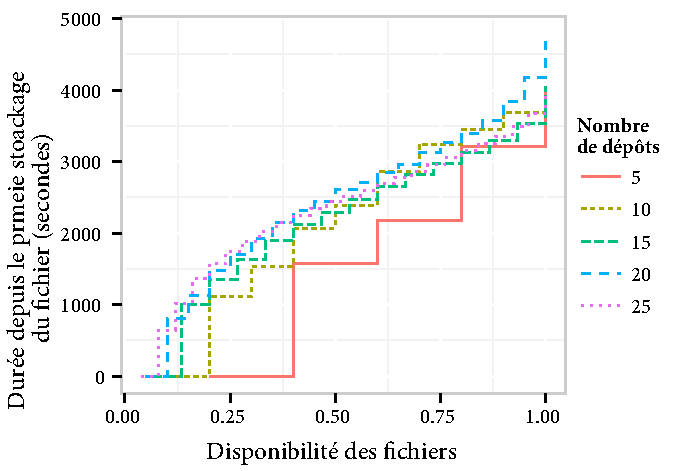
\includegraphics[width=7cm]{figures-fr/propagationTimes-fr.pdf} 
    \caption{Durée de la distribution en fonction de la disponibilité des fichiers dans le système pour différents nombres de dépôts.} 
    \label{fig:propagationTimes-fr} 
    % ggplot(p, aes(x=V3,colour=as.factor(V1),shape=as.factor(V1), linetype=as.factor(V1),y=V4)) + geom_step() + xlab("Proportion of file availability") + ylab("Duration since put time") 
%\end{figure} 
\end{wrapfigure} 
\paragraph{Durée de la distribution.} La première métrique de performance que nous évaluons est le temps nécessaire pour distribuer un fichier dans tous les dépôts. La Figure~\ref{fig:propagationTimes-fr} montre la durée moyenne pour distribuer un fichier en fonction de la disponibilité des fichiers dans le système. Celle-ci est mesurée à partir de l’instant où le fichier est stocké dans le premier dépôt, jusqu’à l’instant où il est distribué à tous les autres dépôts. À noter que le premier dépôt où le fichier est stocké peut être n’importe quel dépôt disponible. 
 
La durée moyenne pour distribuer un fichier, quelque soit le nombre de dépôts disponibles est de environ 4~000~secondes, soit un peu plus d’une heure. Cela prend plus de temps pour distribuer les fichiers au début, avec une seule copie disponible. Avec plus de dépôts qui ont une copie, plus de copies du fichier sont distribuées et la disponibilité augmente plus rapidement. Enfin, notons que cela prend plus de temps pour atteindre le dernier dépôt, puisque c’est généralement le plus éloigné du dépôt de la première copie. 
 
 
Sur la Figure~\ref{fig:propagation-times-matrix-fr}, nous donnons une matrice origine-destination montrant le temps de trajet moyen en minutes entre n’importe quelle paire de dépôts (le nombre de sauts empruntés par le fichier n’est pas représenté). Cela se traduit par la durée moyenne pour distribuer un fichier une fois le fichier stocké dans un dépôt (ce temps prend également en compte les attentes entre deux bus successifs s’il y a un ou plusieurs sauts intermédiaires). Notons que la connectivité des dépôts entre eux dépend du nombre et de la fréquence des trajets en bus les reliant. À titre d’exemple, les dépôts 1 et 15 sont très bien connectés entre eux et disposent d’un temps de trajet moyen inférieur à la moyenne. Ce n’est pas le cas du dépôt 9 qui est plus éloigné du reste, ce qui explique pourquoi cela prend plus longtemps que la moyenne pour y distribuer des fichiers.  
 
 
 
 
\subsection{Migration de machines virtuelles dans des réseaux véhiculaires} 
 
 
Dans cette section, nous présentons le problème de la virtualisation des ressources véhiculaires dans le cadre d’un réseau mobile large-échelle. En particulier, nous nous intéressons à la migration de machines virtuelles déclenchées par des réallocations des ressources virtuelles ou des changements dans la topologie physique (\eg un véhicule ne participe plus à la virtualisation). Afin d’exécuter la phase de migration, au lieu d’utiliser les connexions cellulaires de type 3G ou 4G, nous proposons d’utiliser les communications de véhicule-à-véhicule. Ainsi, nous étudions la caractérisation des opportunités de ``contacts'' entre bus (\ie lorsque deux bus entrent tous deux dans la portée de communication de chacun) dans un contexte urbain large-échelle. 
 
 
Ce travail s’inscrit dans les résultats présentés pour des réseaux similaires de différentes villes, par exemple San Francisco aux États-Unis et Varsovie en Pologne, où les auteurs ont montré que les véhicules entrent en contact plus souvent et pour des durées plus longues à des endroits bien précis~\cite{sarafijanovic2006island}. Ainsi, en limitant les migrations de machines virtuelles à ces endroits, ou ``zones'', nous espérons une amélioration des migrations de machines virtuelles. Nous présentons (\textit{i}) une analyse des opportunités de contacts entre bus de la ville de Dublin en Irlande et (\textit{ii}) une méthodologie similaire à celle présentée dans la Section précédente~\ref{sec:simulation-traces-reelles-fr} pour déterminer ces zones et évaluer les opportunités de migration de machines virtuelles via les communications bus-à-bus. 
 
 
\subsubsection{Génération d’une carte de points chauds des densités de contact} 
 
 
Dans cette section, nous présentons une méthodologie nous permettant dans un premier temps de générer une carte de points chauds représentant les variations spatiales des densités de contacts entre les bus. Dans un second temps, nous déterminons les emplacements des zones avec des durées et fréquences de contacts entre bus plus importantes qu’ailleurs sur la carte. 
 
 
\begin{figure}[t!] 
\centering 
  \begin{subfigure}[t]{0.45\textwidth} 
    \centering 
    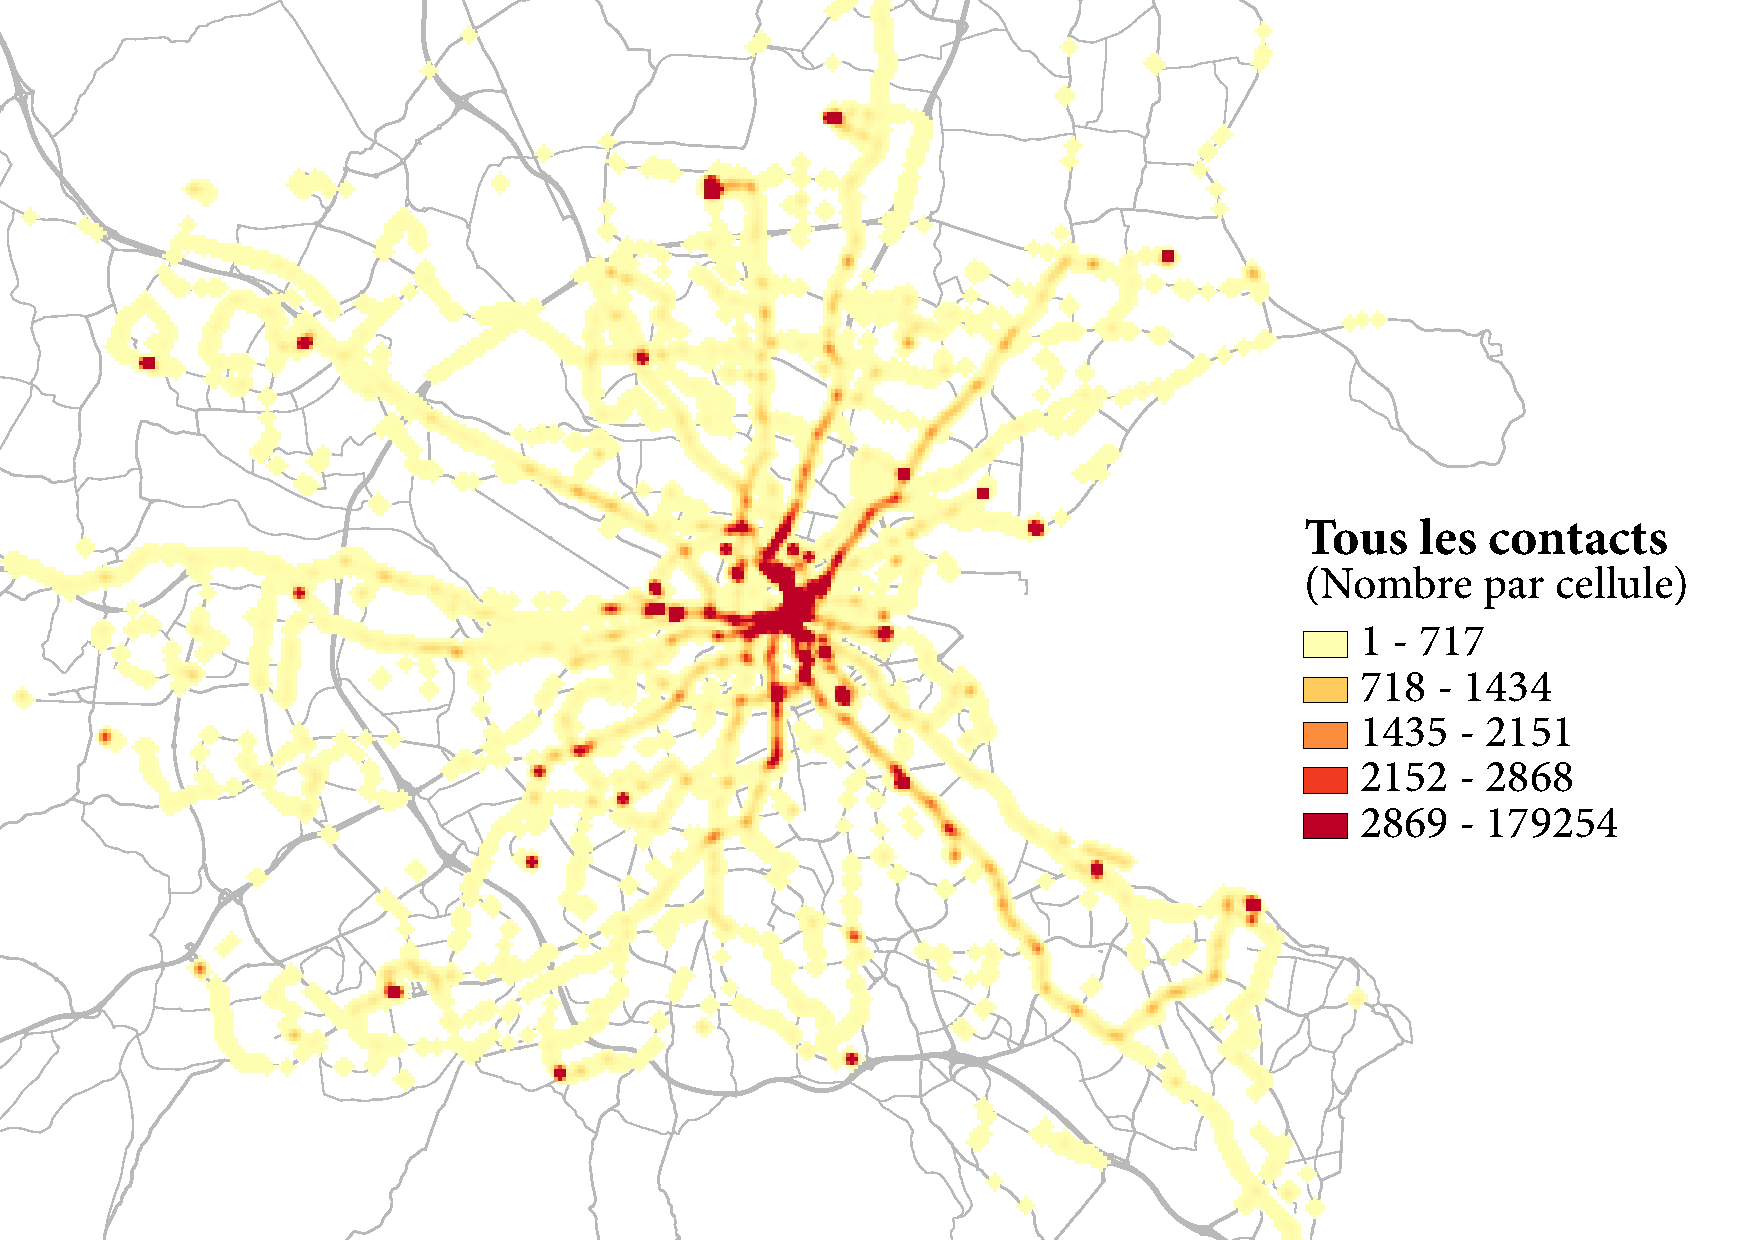
\includegraphics[width=.8\linewidth]{figures-fr/dublin-all-contacts-fr.pdf} 
    \caption{Carte de points chauds de tous les contacts entre bus, quelle que soit leur durée.\vspace{1em}} 
    \label{fig:2d-all-contacts-fr} 
  \end{subfigure}% 
 \qquad 
  \begin{subfigure}[t]{.45\textwidth} 
    \centering 
    \includegraphics[width=.8\linewidth]{figures-fr/dublin-200-contacts-res-fr.pdf} 
    \caption{Carte de points chauds des contacts de durée supérieure à 200 secondes. Les points chauds représentés par des cercles rouges contiennent des cellules dont la densité de contacts est dans le top 25\%.} 
    \label{fig:2d-200-contacts-fr} 
  \end{subfigure} 
 \caption{Carte de points chauds des contacts entre les bus de Dublin en Irlande. La figure montre le nombre de contacts par cellule de taille  100~m $\times$ 100~m.} 
 \label{fig:2d-contacts-fr} 
\end{figure} 
 
 
\paragraph{Carte de points chauds de contacts.} 
La première étape consiste à calculer les variations spatiales des densités de contacts entre bus. Pour ce faire, la carte est divisée en une grille de cellules carrées de taille 100~m $\times$ 100~m. Pour chaque cellule, nous associons la densité de contacts qui occurrent dans la zone géographique de la cellule. Nous représentons la carte de points chauds montrant la densité de contacts sur la Figure~\ref{fig:2d-all-contacts-fr}. Cependant, nous nous intéressons à la migration de machines virtuelles entre bus. Or une machine virtuelle peut avoir une taille relativement importante, nécessitant un transfert de longue durée entre bus. Ainsi, nous représentons sur la Figure~\ref{fig:2d-200-contacts-fr} la carte de points chauds des densités de contacts entre bus d’une durée supérieure ou égale à 200~secondes, pouvant alors transférer une machine virtuelle de taille 200~Mégaoctets avec un débit de 1~Mégaoctet par seconde. Nous utilisons une estimation par noyau (\textit{kernel density estimation} en anglais) pour représenter les cellules ayant une haute signification statistique de leur densité de contacts.  
 
 
Les cartes de points chauds pour la ville de Dublin représentées sur les Figures~\ref{fig:2d-all-contacts-fr} et \ref{fig:2d-200-contacts-fr} montrent les densités de contacts entre bus en utilisant différentes teintes de rouge, les teintes plus foncées indiquant une densité plus élevée de contacts. Notons que les contacts sont surtout concentrés dans le centre ville, mais aussi en périphérie, où les bus terminent généralement leur service.  
 
 
\paragraph{Zones de contact.} 
La deuxième étape consiste à déduire les zones de contact à partir de la carte de points chauds des densités de contacts. Dans un premier temps, nous ordonnons les cellules de la carte de points chauds selon leur densité de contacts. Afin d’exclure les cellules où le nombre de contacts est négligeable, nous sélectionnons les cellules présentant au moins 25\% des meilleures densités de contacts. Les cellules contiguës sont ensuite agrégées en ce que l’on appelle des ``zones de contacts''. Celles-ci sont représentées par des cercles recouvrant l’ensemble des cellules sélectionnées sur la carte de la Figure~\ref{fig:2d-200-contacts-fr}, pour des cellules mesurant la densité de contacts de durée supérieure ou égale à 200~secondes. Le diamètre des zones de contacts correspond à celui couvrant le plus grand ensemble de cellules contiguës. 
 
 
\paragraph{Caractérisation pour les migrations de machines virtuelles.} 
Nous caractérisons ensuite les zones de contact de la Figure~\ref{fig:2d-200-contacts-fr} par rapport à la migration de machines virtuelles. Pour chaque zone de contacts, nous calculons les deux variables suivantes~: (\textit{i}) le nombre total $n$ de contacts d’une durée supérieure ou égale à 200~secondes et (\textit{ii}) la durée moyenne $x$ entre deux contacts successifs. A partir de ces deux variables, nous calculons un score pour chacun des points chauds de la manière suivante~: $\nicefrac{n}{\max(1,\,x)}$. Ce score mesure la capacité d’une zone a pouvoir traiter fréquemment des transferts nécessitant au plus 200~secondes. Enfin, nous utilisons la méthode d’optimisation de Jenks pour classer les zones de contacts en trois classes de valeurs représentatives. 
 
 
Dans la Figure~\ref{fig:2d-200-contacts-fr}, nous utilisons différentes teintes de couleurs pour représenter les zones de contacts selon leur classe de valeurs. Pour évaluer notre méthodologie, nous sélectionnons deux zones de contacts, chacune appartenant à deux classes différentes. La ``zone de contact 1'' a le meilleur score, ce qui indique des contacts de longue durée et fréquents (les trois autres zones de contacts ont un score similaire). La ``zone de contact 2'' est sélectionnée arbitrairement parmi les autres zones ayant un score similaire. 
 
 
\subsubsection{Expérimentation avec des traces réalistes} 
 
 
Dans cette section, nous présentons les résultats des simulations que nous avons faites pour montrer la faisabilité des migrations de machines virtuelles via les communications bus-à-bus. Celles-ci sont présentées pour les bus de la ville de Dublin en Irlande. Plus précisément, nous intéresserons à la capacité des contacts entre bus pour transférer des machines virtuelles de taille variables. 
 
 
\paragraph{Mise en place de l’expérimentation.} 
Nous utilisons un jeu de données publiques des traces de bus de la ville de Dublin, fournies par DublinBus, faisant partie du Dublin City Council. Les traces de mobilité du mois de janvier 2013 donnent les coordonnées GPS estampillées temporellement successives de chaque bus en service opéré par DublinBus~\cite{dublinked}. Nous analysons les mouvements de 823 bus pour le service opéré le 29 janvier 2013 entre 10h et 13h (à heure creuse). Nous supposons que deux bus sont en contact s’il sont chacun dans la portée de communication de l’autre. Pour reproduire les mouvements des bus DublinBus et inférer leurs contacts, nous utilisons le simulateur à évènements discrets ONE pour simuler des interfaces IEEE~802.11 sur les bus~\cite{keranen2009one}. Pour s’affranchir des propriétés de la couche physique telles que le taux d’erreurs binaires, nous considérons une portée de communication de rayon 150~m, volontairement pessimiste avec un débit de 1~Mégaoctet par seconde. 
 
 
\begin{figure}[t!] 
  \centering 
  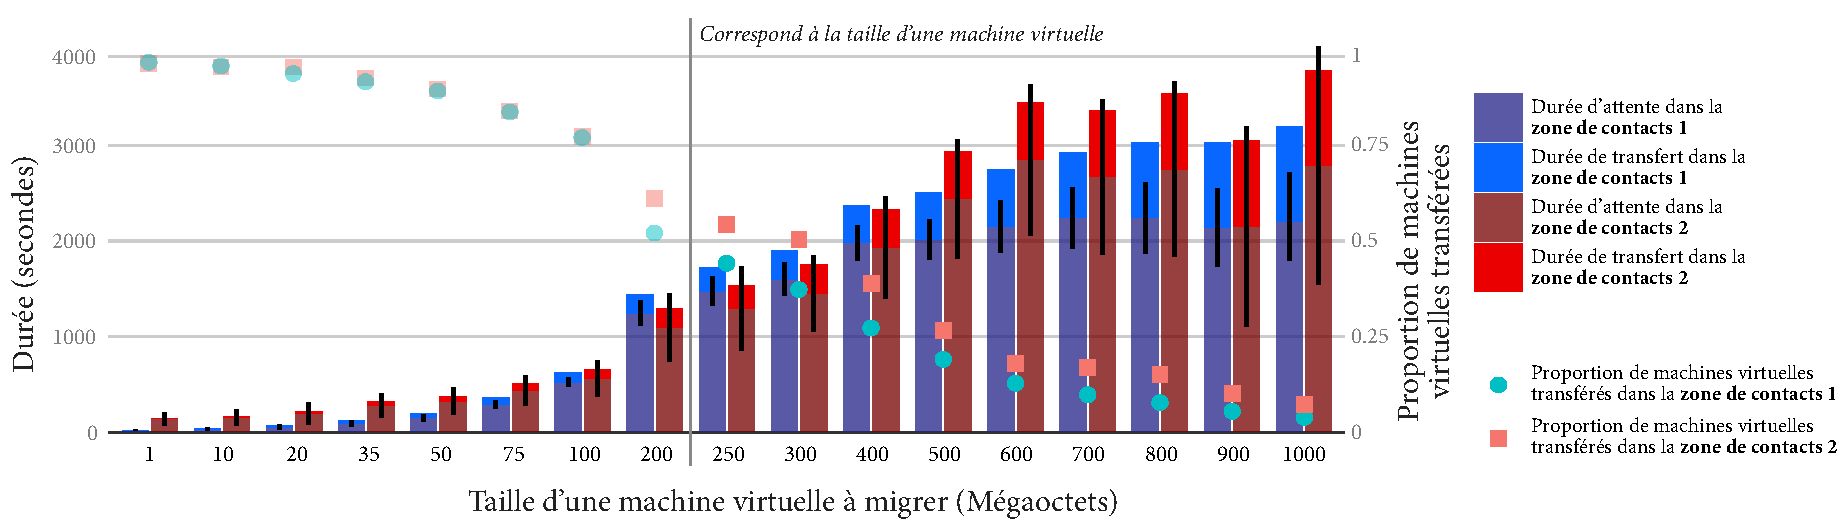
\includegraphics[width=0.98\linewidth]{figures-fr/duration-ratio-migrations-fr.pdf} 
  \caption{Proportion des migrations de machine virtuelle en succès et durée moyenne pour transférer les machines virtuelles en fonction de leur taille. Les barres noires représentent les intervalles de confiance à 95\% du temps d’attente avant de pouvoir transférer avec succès les machines virtuelles.} 
  \label{fig:duration-ratio-migrations-fr} 
\end{figure}  
 
 
Nous simulons les migrations de machines virtuelles pour différentes tailles exécutées par des bus entrant dans les zones de contacts entourées sur la carte de points chauds de Dublin représentée sur la Figure~\ref{fig:2d-200-contacts-fr}. Nous considérons un algorithme de migration naïf qui ne fait aucune supposition ni prédiction sur la future durée des contacts~: lorsqu’un bus entre dans une zone de contacts, celui-ci initie une migration de machine virtuelle avec le premier bus qu’il rencontre. La migration est annulée si la durée du contact n’est pas suffisante pour transférer l’intégralité de la machine virtuelle. 
 
 
Les résultats que nous présentons reflètent les moyennes pour 100 tentatives de migration de machines virtuelles au niveau de chacune des deux zones de contacts. Les différentes tailles que l’on considère représentent les tailles types de machines virtuelles allant de quelques Mégaoctets (\eg TinyOS~\cite{levis2005tinyos}) à plusieurs centaines de Mégaoctets~\cite{clark2005live}. Pour chacune des tailles de machine virtuelle, nous mesurons la durée moyenne nécessaire pour qu’un bus qui entre une zone de contact trouve un contact qui durera suffisamment longtemps pour transférer la machine virtuelle. Le graphe de la Figure~\ref{fig:duration-ratio-migrations-fr} montre la durée moyenne à attendre avant de transférer des machines virtuelles de tailles différentes, ainsi que la proportion de machines virtuelles qui ont pu être transférées parmi toutes les migrations initiées. 
 
\begin{wrapfigure}[11]{o}[0.3\marginparwidth]{8.2cm} 
    \centering 
    \vspace{-14pt} 
    \includegraphics[width=8cm]{figures-fr/contact-durations-histogram-fr.pdf} 
    \caption{Nombre de contacts (avec une échelle logarithmique) pour différents intervalles de durées et leur ratios respectifs (en pourcentage) par rapport au nombre total de contacts dans les zones de contacts 1 et 2.} 
    \label{fig:plot-contact-duration-ratio-fr} 
%\end{figure} 
\end{wrapfigure} 
Tout d’abord, nous remarquons que le ratio de machines virtuelles migrées avec succès décroit avec leur taille, et ce pour chacune des deux zones de contact. Ceci est dû au faible nombre de contacts de longue durée entre les bus, nombre qui décroit avec la durée des contacts. En effet, les bus échouent plusieurs fois avant de trouver un contact qui leur permettra de transférer la machine virtuelle. Cette observation est confirmée par la durée à attendre un ``bon'' contact pour des machines virtuelles de grandes tailles. En général, cela prend moins de temps à trouver un ``bon'' contact au niveau de la zone de contacts 1 qu’au niveau de la zone de contacts 2, sauf pour les machines virtuelles dont la taille est comprise entre 200 et 400~Mégaoctets. 
 
 
Pour expliquer cette tendance, nous représentons dans la Figure~\ref{fig:plot-contact-duration-ratio-fr} le nombre total de contacts mesuré pour différentes durées de contacts ayant lieu dans les zones de contacts 1 et 2. Nous pouvons constater que la zone de contacts 2 a un ratio plus élevé  de contacts de durées comprises entre 200 et 400~secondes. Malgré leur plus grand nombre dans la zone de contacts 1, la plupart d’entre eux ne peuvent pas transférer des tailles de machines virtuelles comprises entre 200 et 400~Mégaoctets. Les bus passent alors plus de temps dans la zone de contacts 1 à essayer de transférer de grandes quantités de données qui vont le plus souvent échouer avant de trouver un ``bon'' contact. Cela explique aussi pourquoi le ratio de migration de machines virtuelles est meilleur dans la zone de contacts 2 lorsque le machines virtuelles ont des tailles comprises entre 200 et 400~Mégaoctets. 

\section{Conclusions} 
 
 
Le travail présenté dans cette thèse se repose sur la mobilité d’entités de tous les jours, et plus particulièrement, celles des voitures particulières et des bus, afin de s’affranchir des limitations et de la dépendance vis-à-vis des réseaux de données traditionnels. Tout au long de cette thèse, nous avons exploité cette mobilité dans le contexte de différentes applications, dont le délestage massif de données et des services véhiculaires de type ``cloud''. 
 
 
\paragraph{Délestage de données massif.} 
Nous avons équipé des véhicules particuliers avec des capacités de stockage connectant des endroits spécifiques que nous avons appelé ``point de délestage''. Ils permettent de capturer d'avantage de trajets que seulement ceux qui effectuent le trajet complet entre la source et la destination d’un transfert de données. Ces points de délestage aident à maximiser les ressources véhiculaires, c’est-à-dire, l’utilisation de l’espace de stockage combiné des véhicules connectant les points de délestage. Pour ce faire, ils jouent le rôle de relais où les trajets des véhicules s’y arrêtant sont composées en un seul chemin logique suivi par le cargo de données qu’ils transportent. Dans la suite, nous détaillons comment nous avons utilisé ces points de délestage pour contrôler et configurer les mouvements des véhicules afin de satisfaire les besoins des transferts de données. 
 
 
\paragraph{Contrôle et configuration de l’infrastructure de délestage.} 
Les points de délestage sont également équipés de capacités de stockage où les cargos de données sont temporairement stockés et passés de manière asynchrone d’un véhicule à l’autre. Ils sont placés là où les véhicules s’arrêtent suffisamment longtemps pour transférer de grandes quantités de données, par exemple dans les parkings situés le long des routes ou ceux situés dans des villes ou des supermarchés, ou encore des stations-services d’essence ou de chargement de batteries électriques. Nous avons proposé une architecture de type SDN (\textit{Software-Defined Networking}) comprenant un contrôleur centralisé qui a une vue globale de l’infrastructure de délestage. Le contrôleur configure les ressources véhiculaires de cette infrastructure à l’aide du réseau de délestage, une représentation logique en quantité réseau des flots de véhicules entre les points de délestage. Plus précisément, ce réseau comporte des liens caractérisés par une capacité, un temps de trajet moyen et un taux d’erreur. Le contrôleur utilise ce réseau de délestage pour résoudre le problème d’allocation de flots de véhicules, qui consiste à sélectionner les chemins logiques du réseau de délestage et à assigner (allouer) des quantités de données sur chacun de ces chemins de façon à satisfaire les besoins spécifiques aux transferts de données. La résolution du problème d’allocation maximise l’utilisation des ressources tout en garantissant une équité entre les allocations des transferts. Son résultat est traduit en règles pour configurer les points de délestage. Ces règles permettent de sélectionner les cargos de données à charger sur les véhicules à l'arrêt. Nos résultats sur le réseau routier français avec des comptages de trafic réels ont permis de montrer que cette architecture centralisée permet d’effectuer une allocation efficiente et équitable des ressources pour des transferts de données en compétition entre des grandes villes de France. 
 
 
\paragraph{Système de stockage et partage véhiculaire.} 
Nous avons exploité le stockage des points de délestage pour les transformer en dépôts où des utilisateurs mobiles peuvent stocker et récupérer des fichiers. Le système repose sur un ensemble de dépôts et les mouvements de utilisateurs entre ceux-ci pour distribuer les fichier dans l’ensemble du système. Nous proposons un algorithme de placement qui permet de déterminer les emplacements optimaux des dépôts de telle sorte que chaque dépôt puisse satisfaire les requêtes des utilisateurs pour stocker ou récupérer des fichiers. Le placement des dépôts prend également en compte les mouvements des utilisateurs afin que les fichiers soient synchronisés entre les dépôts du système sans avoir à recourir à un réseau de données. Nous avons montré que la distribution des fichiers en utilisant le mouvement des utilisateurs mobiles a permis d’augmenter le taux de succès des requêtes. 
 
 
\paragraph{Réseaux véhiculaires virtuels.} 
Nous avons dématérialisé les points de délestage dans le contexte de réseaux véhiculaires où les ressources hébergées par les véhicules (\ie calcul, stockage et communications) sont virtualisées avec des machines virtuelles. Nous avons étudié les migrations de machines virtuelles par des communications véhicule-à-véhicules au lieu de réseau de données de type cellulaires. Dans ce contexte, les points de délestage correspondent aux zones où les véhicules sont fréquemment en contact pour des durées suffisamment longues de manière à pouvoir transférer de grandes quantités de données. Nous avons montré que restreindre les migrations de machines virtuelles à ces zones a permis d’améliorer le taux de succès des migrations de machines virtuelles. 
 
 
Pour résumer et conclure, les points importants de cette thèse sont les suivants~: 
\begin{itemize} 
 
    \item Les véhicules en circulation constituent une ressource avec un potentiel encore inexploité pour transporter des données. Nous avons illustré cette affirmation en simulant des véhicules transportant des données sur les routes françaises et nous avons montré que le réseau routier a le potentiel de transporter plusieurs Pétaoctets de données par jour. 

    \item Une infrastructure dédiée augmente la capacité du système en composant les trajets des véhicules et en configurant le chemin suivi par les données. 

    \item Un contrôle centralisé de l’infrastructure bénéficiant d’une vue globale des flots de véhicules permet une gestion et une allocation efficiente des ressources aux transferts de données. 

    \item Une représentation logique des flots de véhicules en quantités réseau permet de pallier à la complexité du réseau routier et rend l’allocation de transfert de données possible. 

    \item La mobilité des entités du quotidien a le potentiel de fournir des services avec une dépendance limitée vis-à-vis des réseaux de données traditionnels. Nous avons illustré cette affirmation en étendant notre système de délestage dans le contexte de services véhiculaires de type ``cloud''. 

\end{itemize} 
 